 


%%%%%%%%%%%%%%%%%%%%%%%%%%%%%%%%%%%%%%%%%%%%%%%%%%%%%%%%%%%%%%%%%%%%%%%
%%%% Re-released for translation 21 June 2023  %%%%%%%%%%%%%%%%%%%%%%%
%%%%%%%%%%%%%%%%%%%%%%%%%%%%%%%%%%%%%%%%%%%%%%%%%%%%%%%%%%%%%%%%%%%%%%%


\nbbbbbb{Endurants: External Domain Qualities}\label{primer-extq.1}
\pos{\minitoc}{}

\pos{%%%%
\noindent
\begynd
\pind This, the present chapter\pos{, as well as Chapter\,\ref{chap2.tex.Preview},}{}
\begynd
\pind is based on Chapter\,4 of \cite{BjornerMonograph2020}.
\pind You may wish to study that chapter for more detail.
\afslut
\afslut

\mnewfoil
}{}
\nysf{%
\begynd
\pind In this and the next \pos{chapter}{lectures} we shall analyse and describe \sfsl{endurants}, that is, the \sfsl{entities}
\begynd
\pind that can be observed, or conceived and described, \nyl as a ``complete
      thing'' \nyl at no matter which given snapshot of time; 
\pind alternatively an entity is endurant \nyl  if it is capable of
      \sfsl{enduring}, that is \sfsl{persist\ysfchg{s}},
      \sfsl{``hold\ysfchg{s } out''}\pos{
      \cite[Vol.\,I, pg.\,656]{OED}}{}.
\afslut
    
\pind This modelling will focus on the 
\begynd
\pind \sort{types} and
\pind \sort{observers}
\afslut of these endurants.
\mnewfoil

\pind On one hand 
\begynd
\pind there are the domain phenomena of endurants.
\afslut
\pind On the other hand 
\begynd
\pind there are means for analysing and describing these.
\afslut
\pind The former are not formalised ``before'', \nyl or as, we analyse and
      describe them.
\pind The latter, `the means', are assumed formalised.
\afslut
\mnewfoil

\bookdefn{Description, I}{ %
\begynd
\pind By a \sort{description} \index{pdefind}{description!external qualities} of the external
      domain qualities
\begynd
\pind we shall mean a pair of informal, narrative, and formal text
\pind which characterises the compound parts of domains:
\pind their sorts, i.e., types, and
\pind the observers, i.e., informal, functions, that \nyl
      ``dissects'' the compound parts into endurants, \nyl
      usually sub-parts \dbsquare
\afslut
\afslut
}

\noindent
\begynd
\pind This chapter explains what is meant by 
\begynd
\pind \sfsl{external qualities}, \index{pconind}{external qualities} 
\pind \sfsl{endurants} and their  \index{pconind}{endurant}
\pind \sfsl{compound parts}. \index{pconind}{compound part}
\afslut
\afslut
\mnewfoil

\pmt{Primary Modelling Tool, I}
\noindent
\begynd
\pind The tool with which we describe  endurants  will be the 
\begynd
\pind \sort{type} and 
\pind \sort{function} 
\afslut concepts of\pos{, in this case,}{} 
\pind the formal specification language \texttt{RSL} \cite{RSL}.\footnotemark
\afslut
\tmp
}\footnotetext{We could have chosen another formal specification
  language: \texttt{VDM} \citevdm, \texttt{Z} \citez, or
  \texttt{Alloy} \cite{alloy}, or other.}

\nbbbbb{Universe of Discourse}\label{Universe of Discourse}

\ysf{\begynd
\pind The first analysis and description of a chosen domain is that of
its universe of discourse.
\afslut}

\bookdefn{Universe of Discourse, UoD}{
\begynd
\pind By a \bbcolor{\pdindextermii{universe of}{discourse}} we shall
      understand
\begynd
\pind the same as the \bbcolor{\pdindextermii{domain of}{interest}},
\pind that is, the \pcindextermi{domain} to be \pcindextermii{analysed
      \&}{described}\dbsquare
\afslut
\afslut
}

\nbbbb{Identification}

\begynd
\pind The \sort{first task} of a domain analyser cum
describer\footnote{\ysf{Henceforth referred to as the domain modeller.}}
\begynd
\pind is to settle upon the domain to be analysed and described.
\pind That domain has first to be given a \sfsl{name}.
\afslut
\afslut

\nbbbb{Naming}

\begynd
\pind A \sort{first decision} is to give a name to the overall domain sort,
 \pos{}{\\ \hspace*{6mm} *} that is, the type of the domain seen as an endurant,
 \pos{}{\\ \hspace*{6mm} *} with that sort, or type, name 
     \pos{}{\\ \hspace*{12mm}} being freely chosen by the domain \ysf{modeller} --
 \pos{}{\\ \hspace*{6mm} *} with no such sort names having been chosen so far\,!
\afslut

\nbbbb{Examples}

\begynd
\pind \sort{Examples of {UoDs}:}{ \label{page:UoD}\pos{}{\LLLL\HHHH}%
\pos{\begynd
  \pind We refer to a number of Internet accessible experimental
      reports \ysf{\cite{icasestudies}} of
    descriptions of the following domains: 
\afslut}{}
\begin{multicols}{2}
\pos{\begin{quote}\begin{itemize}}{}
\item \bmcolor{\sfsl{railways}} \cite{db00:p:ifac,dines-idpt-02,db03:ifac-cts2003}, 
\item \bmcolor{\sfsl{``The Market''}} \cite{dines-kilov-02},
\item \bmcolor{\sfsl{container shipping}}  \cite{db07:container},
\item \bmcolor{\sfsl{Web systems}} \cite{evaKuhn2010},
\item \bmcolor{\sfsl{stock exchange}} \cite{db:tse:2010:www},
\item \bmcolor{\sfsl{oil pipelines}} \cite{2013pipe},
\item \bmcolor{\sfsl{credit card systems}} \cite{BjornerCreditCard2016},
\item \bmcolor{\sfsl{weather information}} \cite{BjornerWeather2016},
\item \bmcolor{\sfsl{swarms of drones}} \cite{BjornerDrones2017},
\item \bmcolor{\sfsl{document systems}} \cite{BjornerDocuments2017},
\item \bmcolor{\sfsl{container terminals}} \cite{BjornerContainer2018}, 
\item \bmcolor{\sfsl{retail systems}} \cite{BjornerRetailer2021},
\item \bmcolor{\sfsl{assembly plants}} \cite{BjornerTesla2021},
\item \bmcolor{\sfsl{waterway systems}} \cite{BjornerRiversCanals2021},
\item \bmcolor{\sfsl{shipping}} \cite{BjornerShipping2021},
\item \bmcolor{\sfsl{urban planning}} \cite{BjornerUrbanPlanningProcesses2017}.
\pos{\end{itemize}\end{quote}}{}
\end{multicols}
}
\afslut

\nbbbb{Sketching}

\begynd
\pind The \sort{second task} of a domain \ysf{modeller} \nyl
      is to develop a \sfsl{rough sketch narrative} of the domain.
\pind The rough-sketching of \ysf{}  a domain \ysf{} is not a trivial matter.
\begynd
\pind It is not done by a committee\,!
\pind It usually requires repeated ``trial sketches''.
\pind To carry it out, i.e., the sketching, \nyl normally requires a
      combination of
\begynd
\pind physical visits to domain examples, if possible;
\pind talking with domain professionals, at all levels; and
\pind reading relevant literature.
\pind It also includes searching the \texttt{Internet} for information.
\afslut
\afslut
\pind We shall show an example next.
\afslut

\mnewfoil

\monoexample{Sketch of a Road Transport System UoD}{\label{eks:SoaRTSUoD}
\begynd
\pind The road transport system that we have in mind consists of
\begynd
\pind a road net and
\pind a set of automobiles (private, trucks, buses, etc.)
\pind such that the road net serves to convey automobiles.
\afslut
\pind We consider the road net to consist of
\begynd
\pind hubs, i.e., street intersections\ysfchg{, } and
\pind links, i.e., street segments between adjacent hubs%
\footnote{\LLLL{This ``rough'' narrative fails to narrate 
  \pos{what hubs, links, vehicles, automobiles are. In presenting it here we rely on
    your a priori understanding of these terms. But that is
    dangerous\,! The danger, if we do not painstakingly narrate and
    formalise what we mean by all these terms, then readers (software
    designers, etc.) may make erroneous assumptions.}{...}}}\dbsquare
\afslut
\afslut}

\nbbbb{Universe of Discourse Description}

The general universe of discourse, i.e., domain, description prompt
can be expressed as follows:

\ddprompt{describe\_Universe\_of\_Discourse}{ddp:UoD}{\label{UniverseOfDiscourse}%
  
\pos{{\bgcolor{\cdlti\ \bgcolor{\texttt{describe\_Universe\_of\_Discourse}} \sort{describer}}}}% 
    {\vspace*{3mm}\HHHH\bgcolor{\texttt{describe\_Universe\_of\_Discourse}} \sort{describer}}
    \vspace*{2mm}
    \label{DS1}
%\RSLatex
%&\bq\sort{Naming:}&
%   type UoD
%&\sort{Rough Sketch:}&
%   Text &\eq&
%\endRSLatex
\bp
\bq\sort{Naming:}\\
\>\ \kw{type} UoD\\
\sort{Rough Sketch:}\\
\>\ \kw{Text} \eq
\ep
}
\noindent
The above \bq\,\rsltext\,\eq\ expresses that the
\texttt{describe\_Universe\_of\_Discourse()} domain describer generates \rsltext.
\mnewfoil
\noindent
Here is another example rough sketch:

\monoexample{A Rough Sketch Domain Description}{% 
\begynd
\pind The example is that of the production of rum,  
      say of a \sort{Rum Production} domain. 
\pind From
\afslut
%\begin{multicols}{2}\sf
\begin{itemize}%{enumerate}\setei
\item \label{rum0010}the sowing, watering, and tending to of sugar cane plants;
\item \label{rum0020}via the ``burning'' of these prior to harvest;
\item \label{rum0030}the harvest;
\item \label{rum0040}the collection of harvest from sugar cane fields to 
\item \label{rum0050}the chopping, crushing, (and sometimes repeated)
  boiling, cooling and centrifuging of sugar cane when making sugar
  and molasses (into A, B, and low grade batches);
\item \label{rum0060}the fermentation, with water and yeast, producing
  a `wash';
\pos{\psno}{\mnewfoil}
\item \label{rum0070}the (pot still or column still) distilling of the
  wash into rum; 
\item \label{rum0080}the aging of rum in oak barrels;
\item \label{rum0090}the charcoal filtration of rum;
\item \label{rum0100}the blending of rum;
\item \label{rum0110}the bottling of rum;
\item \label{rum0120}the preparation of cases of rum for sales/export; and
\item \label{rum0130}the transportation away from the rum distiller of
  the rum\dbsquare
\end{itemize}\rm%\savei\end{enumerate}\rm
%\end{multicols}
}

\pos{\psno}{\mnewfoil}
%\mnewfoil
\noindent\HHHH
\sort{Some \ysfchg{C}omments on \pos{Example\,\ref{A Rough Sketch Domain Description}}{this example}:}
\begynd
\pind Each of the \ysf{itemized} items above is phrased in terms of perdurants.
\begynd
\pind Behind each such perdurant lies some endurant.
\pind That is, in English, \sfsl{``every noun can be verbed'', and vice-versa.}
\pind So we anticipate the transcendence, \nyl from endurants to perdurants.
\afslut
\afslut

\treprikker

\pos{\psno}{\mnewfoil}

\prinmeth{From the ``Overall'' to The Details}{indsnaevring}{%
\begynd
\pind Our first principle, as the first task \nyl in any new domain
      modelling project, is
\begynd
\pind to ``focus'' on the ``overall'',
\pind that is, on the ``entire'',
\pind generic domain\dbsquare
\afslut
\afslut}


\nbbbbb{Entities}\label{sec:Entities}

\vspace*{-5mm}

A core concept of domain modelling is that of an \sfsl{entity}.

\label{ss.entities}%\LLLL
\bookdefn{Entity}{ %\LLLL%
\begynd
\pind By an \pdindextermi{entity} we shall
      understand a \pdindextermi{phenomenon}, i.e., something
\begynd
\pind that can be \pcindextermi{observe}d, i.e., be
\begynd  
\pind seen or touched by humans,
\pind \sfsl{or} that can be \pcindextermi{conceive}d 
\pind as an \pcindextermi{abstraction}  of an entity;
\afslut 
\pind alternatively,
\begynd
\pind a phenomenon is an entity, \sfsl{if it exists, it is
      \pdindextermi{``being''}, 
\pind it is that which makes a \pcindextermi{``thing''} what it is: \nyl
      essence, essential nature}\pos{ \cite[Vol.\,I, pg.\,665]{OED}}{}.
\afslut%
\afslut%
\pind \dbchg{If a {phenomenon} cannot be so \brcolor{observed and described} then it is
      not en entity}\dbsquare
\afslut%
}%
\mnewfoil
\daprompt{is\_entity}{is-entity}{\label{isentity}%
\begynd
\pind The domain analyser analyses ``things'' ($\theta$) into \nyl either
      entities or non-entities.
\pind The method provides the \dap:
\begin{itemize}
\item \bcolor{\texttt{is\_entity}} -- where 
      \texttt{is\_entity($\theta$)} holds if $\theta$ is an entity\dbsquare\,\,\footnotemark
\end{itemize}
\afslut
}
\footnotetext{\HHHH\dbsquare\ marks the end of an analysis prompt definition.}

\pos{}{\vspace*{1cm}}
\noindent\LLLL\HHHH
\begynd
\pind \texttt{is\_entity} is said to be
\begynd
\pind a \sfsl{prerequisite prompt}
\pind for all other prompts.
\afslut
\pind  \isatool{is\_entity}
\afslut

\mnewfoil

\firkantmedtekst{On Analysis Prompts}{%
\noindent
The \bbcolor{\texttt{is\_entity}} predicate function \nyl represents
the first of a number of analysis prompts. 
\begynd
\pind They are ``applied'' by the \label{firma-analysis}
      domain analyser \nyl  to phenomena of domains.
\pind They yield truth
      values, true or false, \nyl  ``left'' in the mind of the domain
      analyser\dbsquare
\afslut
}

\treprikker
\mnewfoil

\noindent
\begynd
\pind We have just shown how the \texttt{is\_entity} predicate prompt
      can be applied to a universe of discourse. 
\pind From now on we shall see prompts being applicable to
      \ysf{increasingly} more analysed entities.
\pind Figure\,\vref{onto.fig2}
      diagrams \nyl  a \bbcolor{domain description ontology} of entities.
\pind That ontology indicates the sub-classes of endurants \nyl for which we
      shall motivate and for which we shall introduce
\begynd
\pind prompts, 
\pind predicates and 
\pind functions.
\afslut
\afslut

\mnewfoil
\hDBfigure{onto}{\pos{10.5}{11}cm}{The Upper Ontology {-- same as Fig.\,\vref{onto.fig0}}}{onto.fig2}

\noindent
\mnewfoil
\begynd
\pind The present \pos{chapter}{lecture} shall focus only 
\begynd
\pind on the external qualities,
\pind that is, on the ``contents'' of the leftmost \ysf{dash-}dotted box.
\afslut
\afslut

%\mnewfoil

\treprikker

\prinmeth{Justifying Analysis along Philosophical Lines}{justify-filosofi}{%
\begynd
\pind The concept of \sfsl{entities} as a main focal point 
\begynd
\pind is justified in \sfsl{Kai S{\o}rlander}'s philosophy%
      \pos{\cite[1994--2022]{kaisorlander1994,kaisorlander1997,kaisorlander2002,kaisorlander2016,kaisorlander2022}}{}. 
\pind Entities are \pos{there}{in that philosophy} referred to as \sfsl{primary objects}.
\pind They are the ones about which we express predicates\dbsquare
\afslut
\afslut}
      
\nbbbbb{Endurants and Perdurants}\label{sec:Endurants and Perdurants}

\prinmeth{Separation of Endurants and Perdurants}{sep-end-per}{%
\begynd
\pind As we shall see in this \primer, \nyl the domain analysis \&
      description method calls \nyl for the separation of 
\begynd
\pind first considering 
\begynd
\pind the careful analysis \& description
\pind of endurants,
\afslut 
\pind then considering
\begynd
\pind perdurants.
\afslut
\afslut
\pind This principle is based on 
\begynd
\pind the transcendental deduction 
\pind of the latter from the former\dbsquare
\afslut
\afslut}

\nbbbb{Endurants}\label{sec:Endurants}

\bookdefn{Endurant}{ %
\begynd
\pind By an \pdindextermi{endurant}, to repeat, we shall
      understand an entity  
\begynd
\pind that can be observed, or conceived and described, \nyl as a ``complete
      thing'' \nyl at no matter which given snapshot of time; 
\pind alternatively an entity is \ysfchg{an } endurant \nyl  if it is capable of
      \sfsl{enduring}, that is\ysfchg{, } \sfsl{persist\ysfchg{s}},
      \sfsl{``hold\ysfchg{s } out''}\pos{
      \cite[Vol.\,I, pg.\,656]{OED}}{}.
\afslut
Were we to ``freeze'' time 
\begynd
\pind we would still be able to observe the entire endurant \eod
\afslut
\afslut
}
\mnewfoil

\monoexample{Natural and Artefactual Endurants}{\pos{}{\LLLL\HHHH}%
  
\noindent
\bmcolor{Geography Endurants:}  \label{eks:geo}
\pos{}{\begin{multicols}{4}}
\begynd
\pind fields,
\pind meadows,
\pind lakes,
\pind rivers,
\pind forests,
\pind hills,
\pind mountains,
\pind et cetera.
\afslut
\pos{}{\end{multicols}}

\noindent
\bmcolor{Railway Track Endurants:} \label{eks:rail}
\pos{}{\begin{multicols}{2}}
\begynd
\pind a railway track,
\pind its net,
\pind its individual tracks,
\pind switch points,
\pind trains,
\pind their individual locomotives,
\pind signals, 
\pind et cetera.
\afslut
\pos{}{\end{multicols}}
\mnewfoil

\noindent
\bmcolor{Road Transport System Endurants:} \label{eks:road}
\pos{}{}%\begin{multicols}{2}}
\begynd
\pind the transport system,
\pind its road net aggregate and the aggregate of automobiles,
\pind the set of links (road segments) and hubs (road intersections)
      of the road net aggregate,
\pind these links and hubs, and
\pind the automobiles.
\afslut
\pos{}{}%\end{multicols}}
}
\mnewfoil

\daprompt{is\_endurant}{is-endurant}{\label{isendurant}%
\begynd%
\pind The domain analyser analyses an entity, $\phi$, \nyl into
      an endurant \nyl as prompted by the \dap:
\begin{itemize}
\item \bcolor{\texttt{is\_endurant}}
       -- $\phi$ is an endurant
       if \bbcolor{\texttt{is\_endurant($\phi$)}} holds\dbsquare
\end{itemize}
\afslut}

\noindent
\begynd
\pind \texttt{is\_entity} is a \sfsl{prerequisite prompt} 
       for \texttt{is\_endurant}.
\pind  \isatool{is\_endurant}
\afslut
\nbbbb{Perdurants}\label{sec:Perdurants}

\bookdefn{Perdurant}{ %
\begynd
\pind By a \pdindextermi{perdurant} we shall understand an
      entity  
\begynd
\pind for which only a fragment exists\pos{}{\\} if we look at or
      touch them\pos{}{\\} at
      any given snapshot in time.
\pind Were we to freeze time we would only see or
      touch \pos{}{\\} a fragment of the perdurant\pos{
      \cite[Vol.\,II, pg.\,1552]{OED}}{} \eod 
\afslut
\afslut
}
\vspace*{-3mm}
\mnewfoil
\monoexample{Perdurants}{\pos{}{\LLLL\HHHH\sl}%
\noindent
\bmcolor{Geography Perdurants:}
\begynd
\pind the continuous changing of the weather (meteorology);
\pind the erosion of coastlines;
\pind the rising of some land area and the ``sinking'' of other land area;
\pind volcanic eruptions;
\pind earthquakes;
\pind et cetera.
\afslut
                                %\mnewfoil
\noindent
\bmcolor{Railway System Perdurants:}
\begynd
\pind the ride of a train from one railway station to another; and
\pind the stop of a train at a railway station \nyl from some arrival time
to some departure time \eod
\afslut
}
\mnewfoil
\daprompt{is\_perdurant}{is-perdurant}{\label{isperdurant}%
\begynd%
\pind The domain analyser analyses an entity $e$ \nyl into
      \ysfchg{a } perdurant\ysfchg{ } \nyl as prompted by the \dap:
\begin{itemize}
\item \bcolor{\texttt{is\_perdurant}}
   -- $e$ is a perdurant
       if \texttt{is\_perdurant($e$)} holds.
\end{itemize}
\pind \texttt{is\_entity} is a
       \sfsl{prerequisite prompt}
       for \texttt{is\_perdurant} \eoap
\afslut
}
\begynd
\pind \isatool{is\_perdurant}
\afslut

\mnewfoil

\treprikker

\noindent
\begynd
\pind We repeat method principle \vref{sep-end-per}:
\afslut

\prinmeth{Separation of Endurants and Perdurants}{sep-end-per2}{%
\begynd
\pind First domain analyse \& describe endurants;
\pind then  domain analyse \& describe perdurants\dbsquare
\afslut}

\nbbbbb{Solids and Fluids}\label{sec:Solids and Fluids}

\begynd
\pind For \sfsl{pragmatic} reasons we distinguish between
\begynd
\pind solids and 
\pind fluids.
\afslut
\afslut

\prinmeth{Abstraction, I}{abstraction1}{%
\begynd
\pind The principle of \textsf{abstraction} is now brought into ``full play'':
\begynd
\pind In analysing \& describing entities the domain \ysf{modeller}
\pind is ``free'' to not consider all facets of entities,
\pind that is, to abstract.
\pos{ We refer to our characterisation of \textsf{abstraction} in Sect.\,\vref{primer:Abstraction}.}{}
\afslut
\afslut}

\nbbbb{Solids}\label{subsect.Solids}

\bookdefn{Solid Endurant}{ 
\begynd
\pind By a \pdindextermii{solid}{endurant} we shall understand an endurant
\pind which is 
\begynd
\pind  separate,  
\pind individual or
\pind  distinct in form or concept,
\afslut
\pind or, rephrasing:
\begynd
\pind  a body 
\pind or magnitude
\afslut
  of three-dimensions, \nyl having length, breadth and thickness
  \cite[Vol.\,II, pg.\,2046]{OED} \eod\ \
\afslut
}

\mnewfoil

\daprompt{is\_solid}{is solid}{\label{issolid}%
\begynd
\pind The domain analyser analyses endurants, $e$, \nyl into solid
      entities \nyl as prompted by the \dap:
\begin{itemize}
\item \bcolor{\texttt{is\_solid}}
      \doanpr\apindex{is\_solid}%
      -- $e$ is solid
      if \texttt{is\_solid($e$)} holds \eoap
\end{itemize}
\afslut
}
\noindent
\begynd
\pind To simplify matters we shall allow \nyl  separate elements of a
      solid endurant to be fluid\,! 
\pind That is, a solid endurant, i.e., a part, \nyl  may be
      conjoined with a fluid endurant, a fluid.
\pind \isatool{is\_solid}
\afslut

\mnewfoil

\monoexample{Artefactual Solid Endurants}{\HHHH%
\begynd
\pind The individual endurants of the above example \nyl of \sort{railway system}
      endurants, Example\,\vref{eks:geo}, \nyl were all solid.
\pind Here are examples of solid endurants of \sort{pipeline systems}.
\begynd
\pind A pipeline and
\pind its individual units:
\pos{}{\begin{multicols}{3}}
\begynd
\pind wells,
\pind pipes, 
\pind valves, 
\pind pumps, 
\pind forks,
\pind joins,
\pind regulator, and 
\pind sinks \eod
\afslut
\pos{}{\end{multicols}}
\afslut
\afslut
}
\nbbbb{Fluids}\label{subsect.Fluids}

\chardefn{Fluid Endurant}{ %
\begynd
\pind By a \pdindextermii{fluid}{endurant} we shall understand \nyl   an endurant which is 
\begynd
\pind prolonged, without interruption, \nyl  in an unbroken series or pattern;
\afslut or, rephrasing:
\begynd
\pind a substance (liquid, gas or plasma)  \nyl 
      having the property of flowing,  \nyl  
      consisting of particles \nyl  
      that move  among themselves \cite[Vol.\,I, pg.\,774]{OED} \eod
\afslut
\afslut
} 
\mnewfoil

\daprompt{is\_fluid}{is fluid}{\label{isfluid}%
\begynd
\pind The domain analyser analyses endurants $e$ into fluid
      entities as prompted by the \dap:
\begin{itemize}
\item \bcolor{\texttt{is\_fluid}} 
      \doanpr\pos{\apindex{is\_fluid}}{}%
      -- $e$ is fluid if \texttt{is\_fluid($e$)} 
      holds \eoap 
\end{itemize}
\afslut
}
\noindent
\begynd
\pind \isatool{is\_fluid}
\mnewfoil
\pind Fluids are otherwise
\begynd
\pind liquid, or
\pind gaseous, or
\pind plasmatic, or
\pind granular\footnote{\label{fn.granular1}\LLLL This is a purely
      pragmatic decision. \nyl ``Of course'' sand, gravel, soil, etc., are not
      fluids, \nyl  but for our modelling purposes it is convenient \nyl  to
      ``compartmentalise'' them as fluids\,!}, or
\pind plant products\footnote{\LLLL i.e., chopped sugar cane, threshed, or
      otherwise. See footnote \vref{fn.granular1}.},
\pind et cetera.
\afslut
\afslut
\mnewfoil

\monoexample{Fluids}{\smallish\HHHH%
\begynd
\pind Specific examples of fluids are:
\begynd
\pind water, oil, gas, compressed air, etc.
\afslut
\pind A container, which we consider a solid endurant,
\begynd
\pind may be \sfsl{conjoined} with another, a fluid, 
\pind like a gas pipeline unit may ``contain'' gas\dbsquare
\afslut
\afslut
}

\nbbbbb{Parts and Living Species}\label{sec:Parts and Living Species}

\begynd
\pind We  analyse endurants into either of two kinds:
\begynd
\pind \sfsl{parts} and
\pind \sfsl{living species}.
\afslut
\pind The distinction between \sfsl{parts} and \sfsl{living species} \nyl
      is motivated in \kaisorfil\
      \cite{kaisorlander1994,kaisorlander1997,kaisorlander2002,kaisorlander2016,kaisorlander2022}. 
\afslut

\nbbbb{Parts}\label{sec:Parts}
   
\bookdefn{Part}{\label{physical-parts-defn}
\begynd
\pind By a \sfsl{part} we shall understand
\begynd
\pind a solid endurant existing in time and
\pind subject to laws of physics,
\pind including the \sfsl{causality principle} and
\pind \sfsl{gravitational pull}\footnotemark \eod
\afslut
\afslut
}\footnotetext{\LLLL This characterisation
  is the result of our study of relations between philosophy and
  computing science, notably influenced by \kaisorfil\
      \cite{kaisorlander1994,kaisorlander1997,kaisorlander2002,kaisorlander2016,kaisorlander2022}\label{influencex}}
\mnewfoil

\newestdaprompt{is\_part}{is physical part}{e}{part}{a part}{isphysicalpart}

\noindent
\isatool{is\_part}
\mnewfoil
\begynd
\pind \ysf{} \sfsl{Parts} are
\begynd
\pind either \sfsl{natural} parts, or are
\pind \sfsl{artefactual} parts, i.e. man-made.
\afslut
\pind Natural and man-made parts are either
\begynd
\pind \sfsl{atomic} or
\pind \sfsl{compound}.
\afslut
\afslut
\mnewfoil
      
\nbbb{Atomic Parts}\label{sec:Atomic Parts}

\begynd
\pind The term `atomic' is, perhaps, misleading.
\begynd
\pind It is not used in order to refer to nuclear physics.
\pind It is, however, chosen in relation to the notion of
      \sfsl{atomism:}
\begynd
\pind \sl a doctrine that the physical or physical and mental universe 
\pind is composed of simple indivisible minute particles \rm\merriam.
\afslut
\afslut
\afslut

\bookdefn{Atomic Part}{ \label{px-atomic}
\begynd
\pind By an \sfsl{atomic part} we shall understand a part
\begynd
\pind which the domain analyser considers to be indivisible
\pind in the sense of not meaningfully \ysfchg{divisible},
\pind for the purposes of the domain under consideration,
\pind that is, to not meaningfully consist of sub-parts\eod
\afslut
\afslut
}

\mnewfoil

\monoexample{Some Atomic Parts}{
\begynd
\pind We refer to Example\,\vref{Artefactual Solid Endurants}:
  pipeline systems. The
\begynd
\pind wells,
\pind pumps, 
\pind valves, 
\pind pipes, 
\pind forks, 
\pind joins and 
\pind sinks
\afslut can be considered atomic\dbsquare
\afslut}

\mnewfoil
\newestdaprompt{is\_atomic}{is atomic part}{e}{atomic part\ysfchg{s }}{an atomic part}{isatomicpart}

\noindent
\isatool{is\_atomic}

\mnewfoil%\pos{}{\newpage}

\nbbb{Compound Parts}\label{sec:Compound Parts}

\begynd
\pind We, pragmatically, distinguish between
\begynd
\pind Cartesian-product-, and 
\pind set-
\afslut oriented  parts.
\pind That is, if Cartesian-product-oriented, \nyl to consist of two or more \nyl
      distinctly sort-named endurants (solids or fluids),
\pind or, if set-oriented, \nyl to consist of an indefinite number of zero,
      one or more \nyl identically sort-named parts.
\afslut

\mnewfoil

\bookdefn{Compound Part}{ %
\begynd
\pind \pdindextermii{Compound}{part}s are those which
\begynd
\pind either \ysfchgii{are } Cartesian-product-
\pind or are set-
\afslut
\pind oriented parts  \eod
\afslut
}

\mnewfoil


\newestdaprompt{is\_compound}{is compound part}{e}{compound part\ysfchg{s }}{a
  compound part}{iscompoundpart}

\noindent
\isatool{is\_compound}

\nbb{Cartesian Parts}\label{sec:Composite Parts}

\bookdefn{Cartesian Part}{
\begynd
\pind A \pdindextermii{Cartesian}{part} \ysfchg{is a compound part }
\begynd
\pind which consists of an ``indefinite number'' 
\pind of two or more parts 
\pind of distinctly named sorts\dbsquare
\afslut
\afslut
}

\pos{%%%%%%%%%%%%%%%%
\noindent
\begynd
\pind Some clarification may be needed.
\begynd
\pind (i) In mathematics, as in \texttt{RSL} \citersl, 
\begynd
\pind a value is a Cartesian value 
\pind if it can be expressed, for example as $(a,b,...,c)$,
\pind where $a, b, ..., c$ are mathematical (or, which is the same, \texttt{RSL}) values.
\pind Let the sort names of these be $A, B, ..., C$ --
\pind with these being required to be distinct.
\pind We wrote ``indefinite number'':
\begynd
\pind the meaning being that the number is fixed, finite, but not specific.
\afslut
\afslut
\afslut
\pind (ii) The requirement: `distinctly named' is pragmatic.
\begynd
\pind If the domain \ysf{modeller} thinks 
\pind that two or
      more of the components of a  Cartesian part 
\pind are [really] of the same sort, 
\pind then that person is most likely confused
\pind and must come up with suitably distinct sort names for these
      ``same sort'' parts\,!
\afslut
\pind (iii) Why did we not write ``definite number''\,?
\begynd
\pind Well, at the time of first analysing a Cartesian part,
\pind the  domain \ysf{modeller} 
\pind may not have thought of all the consequences, i.e., analysed,
\pind the compound part.
\pind Additional sub-parts, of the Cartesian compound, may be
      ``discovered'', subsequently
\pind and can then, 
\pind with the approach we are taking \ysfchg{with respect to } the modelling of these,
\pind be ``freely'' added subsequently\,!
\afslut
\afslut
}{}

\mnewfoil

\monoexample{Cartesian Automobiles}{\HHHH%
\noindent
\begynd
\pind We refer to Example\,\vref{eks:road}, \nyl the \ysf{transport
  system} sub-example.
\pind We there viewed (hubs, links and) automobiles \nyl as atomic parts.
\pind From another point of view \nyl we shall here understand automobiles \nyl
      as Cartesian parts:
\pos{}{\begin{multicols}{2}}
\begynd
\pind the engine train,
\pind the chassis,
\pind the car body,
\pind four doors (left front, left rear, right front, right rear), and
\pind the wheels.
\afslut
\pos{}{\end{multicols}}
\pind These may again be considered Cartesian parts.
\afslut
}

\mnewfoil


\newestdaprompt{is\_Cartesian}{is-cartesian}{e}{Cartesian
  part\ysfchg{s }}{a
  Cartesian part}{iscartesian}

\noindent
\isatool{is\_Cartesian}

\nspb{Determine Cartesian Part Sorts}\label{descr.Compounds.Composites}

\begynd
\pind The above analysis amounts to the analyser 
\begynd
\pind first ``applying'' the \sfsl{domain analysis} prompt
\pind \texttt{is\_\-com\-pound}($e$)
      to a solid endurant, $e$,
\pind where we now assume that the obtained truth value is \keyw{true}. 
\pind Let us assume that endurant\ysfchg{ } $e$:$E$ consist\ysfchg{s } of sub-endurants of
      sorts \pos{}{\\} $\{E_{1}$,\-$E_{2}$,\-\ldots,\-$E_{m}\}$.
\pind Since we cannot automatically guarantee that our domain
      descriptions secure that
\pind \textsf{E} and \ysfchg{all these } \textsf{E$_i$}
      (\textsf{1{\LEQ}$i${\LEQ}m}) 
\pind denotes disjoint sets of entities 
      \ysf{\sfsl{we must prove so\,!}}
\afslut
\afslut

\treprikker

\mnewfoil

\firkantmedtekst{On Determination Functions}{
\label{firma-observex}%
\vspace*{1mm}  
\noindent
\begynd
\pind Determination functions
\begynd 
\pind apply to compound parts
\pind and yield their sub-parts and the sorts of these.
\afslut
\pind \sfsl{That is,
\begynd
\pind we observe the domain
\pind  and our observation results
\pind  in a
      focus on a subset of that domain
\pind  and 
      sort information about that subset.
\vspace*{1mm} 
\afslut}
\afslut}

\mnewfoil

\noindent
\firkantmedtekst{An RSL Extension}{\label{An RSL Extension}{\LLLL\HHHH%%%
\noindent
\begynd
\pind The \textsf{determine\_$\cdots$} functions below are expressed as follows:

%\RSLatex
%   value determine_&$\cdots$&(e) as (parts,sorts)
%\endRSLatex 
\bp
\>\ \kw{value} determine\_$\cdots$(e) \kw{as} (parts,sorts)
\ep


\noindent
\begynd
\pind where we focus here on the \textsf{sorts} clause.
\pind Typically that clause is of the form
\textsf{$\eta$A,$\eta$B,...,$\eta$C}. \footnotemark
\pind That is, a ``pattern'' of sort names: \textsf{A,B,...,C}.
\afslut
\pind These sort names are provided by the domain \ysf{modeller}.
\pind They are chosen as ``full names'', or as mnemonics, \nyl to
      capture an essence of the (to be) described sort.
\pind Repeated invocations, by the  domain \ysf{modeller},
      \nyl of these \textsf{(...,sorts)} analysis functions normally \nyl lead to new sort
      names \nyl distinct from previously chosen such names.
\afslut
}}\footnotetext{\LLLL
    \textsf{$\eta$A,$\eta$B,...,$\eta$C} are \bbcolor{names} of
    types. $\eta\theta$ is the type of all type names\,!}


\dafprompt{determine\_Cartesian\_part\_sorts}{analyse-cp}{\label{determineCartesian}%%
\begynd%%
\pind The domain analyser analyses a part  into a Cartesian part.
\pind The method \ysf{thus} provides the \dop:
\begin{itemize}
\item \bcolor{\texttt{determine\_Cartesian\_part\_sorts}}
     --- it directs the domain analyser  \nyl to determine the definite
      number of values  \nyl and corresponding distinct sorts of the part.
%\RSLatex
%value
%    determine_Cartesian_part_sorts: E -> (E1><E2><...><En) >< (&$\eta$&E1><&$\eta$&E2><...><&$\eta$&En)&\footnotemark&
%    determine_Cartesian_part_sorts(e) as ((e1,...,en),(&$\eta$&E1,...,&$\eta$&En))
%\endRSLatex 
\bp
\kw{value}\\
\>\>determine\_Cartesian\_part\_sorts: E {\RIGHTARROW} (E1{\TIMES}E2{\TIMES}{\DOTDOTDOT}{\TIMES}En) {\TIMES} ($\eta$E1{\TIMES}$\eta$E2{\TIMES}{\DOTDOTDOT}{\TIMES}$\eta$En)\footnotemark\\
\>\>determine\_Cartesian\_part\_sorts(e) \kw{as} ((e1,{\DOTDOTDOT},en),($\eta$E1,{\DOTDOTDOT},$\eta$En))
\ep
\noindent
where by \textsf{E, Ei} we mean endurants, i.e., part values, and by
\textsf{$\eta$Ei} we mean the names of the corresponding types  \eoap
\end{itemize}
\afslut}\footnotetext{\LLLL The ordering,
\textsf{((e1,...,en),{($\eta$E1,{\DOTDOTDOT},$\eta$En)})}, is pairwise
arbitrary.}
\noindent

%\pos{\psno}{\mnewfoil}
\noindent
\isatool{determine\_Cartesian\_part\_sorts}

\mnewfoil

\noindent
\firkantmedtekst{On Calculate Prompts}{\noindent \label{firma-observey}%
\begynd
\pind Calculation prompts
\begynd 
\pind apply to compound parts: Cartesians and sets,
\pind and yield an \rsltxt\ description.
\afslut
\afslut}

\pos{\psno}{\mnewfoil}

\noindent
\nspb{Describe Cartesian Part Sorts}\label{sec:Analyse Composite Parts}\LLLL

\ddprompt{describe\_Cartesian\_part\_sorts}{calc-Cartesian-parts}{ \label{DS2}\label{calcCartesianParts}%
\begynd
\pind If \texttt{is\_Cartesian}($e$) holds, then the analyser 
      ``applies'' the \ddp\
\begin{itemize}
\item \bgcolor{\texttt{describe\_Cartesian\_part\_sorts}($e$)}
      \dpindex{describe\_Cartesian\_part\_sorts}%
\end{itemize}
\noindent
resulting in the analyser writing down \nyl
the \ysf{\ddtu{endurant sorts and endurant sort observers}}\
\afslut

\pos{\psno\vspace*{2mm}}{\mnewfoil}\label{nar+for-1}

\bdbrule

\pos{{\bgcolor{\cdlti\ \bgcolor{\texttt{describe\_Cartesian\_part\_sorts(e)}}:}}}% 
    {\vspace*{3mm}\HHHH\bgcolor{\texttt{describe\_Cartesian\_part\_sorts}}:}
    %\delati{describe\_Cartesian\_part\_sorts}
    \vspace*{2mm}\LLLL\HHHH
%\RSLatex
%   let (_&\footnotemark&,(&{$\eta$E$_1$,...,$\eta$E$_m$}&)) = determine_Cartesian_parts(e)&\footnotemark\ & in&\afindex{determine\_Cartesian\_part\_sorts}&
%&\bq\kw{Narration:}& 
%   [s]   ... narrative text on sorts ...
%   [o]   ... narrative text on sort observers ...
%   [p]   ... narrative text on proof obligations ...
%&\kw{Formalisation:}&
%   type
%   [s]   E&$_1$&, &\eq& ...&\bq&, E&$_m$&
%   value
%   [o]   &{\obs}&E&$_1$&: E -> E&$_1$&,&\eq ...\bq&, &{\obs}&E&$_m$&: E -> E&$_m$& &\delaoi{\protect{\obsmoe}}\label{obsmoestrux}\label{obsmoeendx}&
%   &\kw{proof obligation}&
%   [p]   [ Disjointness &of& endurant sorts ]&\eq\label{parts-postrux}&
%   end
%\endRSLatex
\bp
\>\ \kw{let} ({\UNDERLINE}\footnotemark,({$\eta$E$_1$,...,$\eta$E$_m$})) {\EQ} determine\_Cartesian\_parts(e)\footnotemark\  \kw{in}\afindex{determine\_Cartesian\_part\_sorts}\\
\bq\kw{Narration:} \\
\>\ {\LBRACKET}s{\RBRACKET}\ \ \ {\DOTDOTDOT} narrative text on sorts {\DOTDOTDOT}\\
\>\ {\LBRACKET}o{\RBRACKET}\ \ \ {\DOTDOTDOT} narrative text on sort observers {\DOTDOTDOT}\\
\>\ {\LBRACKET}p{\RBRACKET}\ \ \ {\DOTDOTDOT} narrative text on proof obligations {\DOTDOTDOT}\\
\kw{Formalisation:}\\
\>\ \kw{type}\\
\>\ {\LBRACKET}s{\RBRACKET}\ \ \ E$_1$, \eq {\DOTDOTDOT}\bq, E$_m$\\
\>\ \kw{value}\\
\>\ {\LBRACKET}o{\RBRACKET}\ \ \ {\obs}E$_1$: E {\RIGHTARROW} E$_1$,\eq ...\bq, {\obs}E$_m$: E {\RIGHTARROW} E$_m$ \delaoi{\protect{\obsmoe}}\label{obsmoestrux}\label{obsmoeendx}\\
\>\ \kw{proof obligation}\\
\>\ {\LBRACKET}p{\RBRACKET}\ \ \ {\LBRACKET} Disjointness of endurant sorts {\RBRACKET}\eq\label{parts-postrux}\\
\>\ \kw{end}
\ep
\edbrule
}
\addtocounter{footnote}{-1}
\footnotetext{\LLLL The use of the underscore, \_\ , shall inform the reader
   that there is no need, here, for naming a value.}
\addtocounter{footnote}{1}
\footnotetext{\LLLL For
  \texttt{determine\_Cartesian\_part\_sorts} see Sect.\,\vref{sec:Analyse
    Composite Parts}}
\noindent
\pos{\psno}{\mnewfoil}
\isatool{describe\_Cartesian\_part\_sorts}

\vspace{1mm}

\noindent
\elaboration{Type, Values and Type Names}{type-values-typenames2}{
\begynd
\pind Note the use of quotes above. 
\pind Please observe that when we write \textsf{obs\_E} \nyl  then
      \textsf{obs\_E} is the name of a function.
\pind The \textsf{E}\ysf{} when juxtaposed to \textsf{obs\_} is now a name  \eod
\afslut}

\ysfchg{ %%%%%%%%%%%%%%%
\dbeat{%%%%%%%%%%%%%%%%
%\pos{\psno}{\mnewfoil}
\dafprompt{type\_name, type\_of, is\_}{type-name1}{\label{name-type}%
The definition of \textsf{type\_name} and \textsf{type\_of}\pos{}{\\} implies the informal definition of
%\RSLatex
%   &obs\_E$_i$&(e)=e&$_i$& is type_name(e&$_i$&)=&\bq{E$_i$}\eq& /\
%   type_of(e&$_i$&) is E&$_i$& /\
%   is_E&$_i$&(e&$_i$&)
%\endRSLatex 
\bp
\>\ obs\_E$_i$(e){\EQ}e$_i$ {\IS} type\_name(e$_i$){\EQ}\bq{E$_i$}\eq {\WEDGE}\\
\>\ type\_of(e$_i$) {\IS} E$_i$ {\WEDGE}\\
\>\ is\_E$_i$(e$_i$)
\ep
}}}%%%%%%%%%%%%%%%%%%%%

\pos{}{\mnewfoil}
\monoexample{A Road Transport System Domain: Cartesians}{\index{eind}{A Road
    Transport Domain!Composite}\pos{\footnotemark}{}
  \pos{\begin{multicols}{2}}{}
\begin{enumerate}\setei
\item \label{x-pts-000} There is the \sfsl{universe of discourse},
      \textsf{RTS}.
\savei\end{enumerate}
\noindent 
It is composed from \ptsidxi{UoD}{x-pts-000}
\begin{enumerate}\setei  
\item \label{x-pts-020} a \sfsl{road net}, \textsf{RN}, and
  \ptsidxi{RN}{x-pts-020} 
\item \label{x-pts-030} an \sfsl{aggregate of automobiles},
  \textsf{AA}. \ptsidxi{AA}{x-pts-030} 
  \savei\end{enumerate}
\pos{\end{multicols}}{}
\noindent
\pos{\begin{multicols}{2}}{}
%\RSLatex
%type
%&\ref{x-pts-000}&  RTS
%&\ref{x-pts-020}&  RN
%&\ref{x-pts-030}&  AA
%value
%&\ref{x-pts-020}&  obs_RN: RTS -> RN &\psfidxi{obs\_RN}{x-pts-020}&
%&\ref{x-pts-030}&  obs_AA: RTS -> AA &\psfidxi{obs\_AA}{x-pts-030}\eox&
%\endRSLatex
\bp
\kw{type}\\
\ref{x-pts-000}\ \ RTS\\
\ref{x-pts-020}\ \ RN\\
\ref{x-pts-030}\ \ AA\\
\kw{value}\\
\ref{x-pts-020}\ \ obs\_RN: RTS {\RIGHTARROW} RN \psfidxi{obs\_RN}{x-pts-020}\\
\ref{x-pts-030}\ \ obs\_AA: RTS {\RIGHTARROW} AA \psfidxi{obs\_AA}{x-pts-030}\eox
\ep
\pos{\end{multicols}}{}
\rm
\pos{\psno}{\mnewfoil}
\noindent
\pos{\begin{multicols}{2}}{}
\begin{enumerate}\setei
\item \label{x-pts-040}  The road net consists of
\begin{enumerate}
\item \label{x-pts-040a} an aggregate, \textsf{AH}, of hubs and
  \ptsidxi{SH}{x-pts-040a} 
\item \label{x-pts-040b} an aggregate,  \textsf{AL}, of
  links. \ptsidxi{SL}{x-pts-040b}  
\end{enumerate}
\savei\end{enumerate}\footsize\HHHH
\pos{\end{multicols}}{}
\pos{\begin{multicols}{2}}{}
%\RSLatex
%type 
%&\ref{x-pts-040a}&  AH
%&\ref{x-pts-040b}&  AL
%value
%&\ref{x-pts-040a}&  obs_AH: RN -> AH  &\psfidxi{obs\_AH}{x-pts-040a}&
%&\ref{x-pts-040b}&  obs_AL: RN -> AL &\psfidxi{obs\_AL}{x-pts-040b}\eod& 
%\endRSLatex
\bp
\kw{type} \\
\ref{x-pts-040a}\ \ AH\\
\ref{x-pts-040b}\ \ AL\\
\kw{value}\\
\ref{x-pts-040a}\ \ obs\_AH: RN {\RIGHTARROW} AH\ \ \psfidxi{obs\_AH}{x-pts-040a}\\
\ref{x-pts-040b}\ \ obs\_AL: RN {\RIGHTARROW} AL \psfidxi{obs\_AL}{x-pts-040b}\eod 
\ep
\normalsize\rm
\pos{\end{multicols}}{}
\pos{\footnotetext{\LLLL In example \vref{A Road Transport System Domain:
      Cartesians}' the \sort{Narration} is not 
    representative of what it should be. Here is a more reasonable
    narration:
\begin{itemize}
\item A road net is a set of \textsf{hubs} (road intersections) and \textsf{links}
such that links are connected to adjacent hubs,
 and such that connected links and hubs form \sfsl{roads}
and where a road \texttt{is a thoroughfare, route, or way on
    land between two places that has been pa\-ved or otherwise improved
    to allow travel by foot or some form of conveyance, in\-cluding a
    motor vehicle, cart, bicycle, or horse \wiki}  
\end{itemize}

We bring this clarification here, once, and allow ourselves, with the
reader's permission, to narrate only very steno-graphically.
}}{}}

\nbb{Part Sets}\label{sec:Part Sets}

\bookdefn{Part Sets}{ %
\begynd
\pind \pdindextermii{Part}{set}s are those \ysf{parts} which,
\begynd
\pind in a given context, 
\pind are deemed to \textsl{meaningfully} consist of \pos{}{\\}
      separately observable 
\begynd
\pind a [``root''] part and
\pind an indefinite number of proper [``sibling''] \termi{sub-part}s\eod
\afslut
\afslut
\afslut
}

\pos{\psno}{\mnewfoil}

\bookdefn{Part Set Sort}{ %
\begynd
\pind \pdindextermi{Part set sort}s are those which,
\begynd
\pind in a given context, 
\pind are deemed to \textsl{meaningfully} consist of \pos{}{\\}
      separately observable 
\begynd
\pind a [``root''] part and
\pind an indefinite number of proper [``sibling''] \termi{sub-part}s of
      the same sort \eod
\afslut
\afslut
\afslut
}

\pos{\psno}{\mnewfoil}

\daprompt{is\_part\_set\_sort}{is-single-sort-set}{\label{issinglesortset}%
\begynd
\pind The domain analyser analyses a solid endurant, i.e., a part
      $p$ into a set endurant:   
\begin{itemize}
\item \bcolor{\texttt{is\_part\_set\_sort}}: $p$ is a
      composite endurant \nyl if \texttt{is\_part\_set\_sort($p$)} holds \eoap
\end{itemize}
\afslut
}

\noindent
\isatool{is\_part\_set\_sort}

\pos{\psno}{\mnewfoil}

\begynd
\pind The \bcolor{\texttt{is\_part\_set\_sort}} predicate is informal. 
\pind So are all the domain analysis predicates (and functions). 
\pind That is,
\begynd
\pind \ysf{t}heir values are ``calculated'' by a human, the domain analyser.
\pind That person observes \ysf{fragments} in the ``real world''.
\pind The determination of the predicate values, hence, are subjective.
\afslut
\afslut

\pos{\psno}{\mnewfoil}

\nspb{Determine Part Set Sort}\label{sec:Analyse
  Same Sorts Part Sets}\label{Single Sort Part Sets}

\dafprompt{determine\_part\_set\_sort}{determine-single-sort-part-set}{ \label{DsSpS}%%
\begynd%%
\pind The domain analyser observes parts into part set sorts.
\pind The method provides the \dop:
\begin{itemize}
\item \bcolor{\texttt{determine\_part\_set\_sort}} \nyl
  directs the domain analyser to determine  the values \nyl and corresponding
      sorts of the part.
%\RSLatex
%value
%    determine_part_set_sort: E -> P-set><&$\theta$&P
%    determine_part_set_sort(e) as (ps,&$\eta$&Pn)
%\endRSLatex 
\bp
\kw{value}\\
\>\>determine\_part\_set\_sort: E {\RIGHTARROW} P\kw{-set}{\TIMES}$\theta$P\\
\>\>determine\_part\_set\_sort(e) \kw{as} (ps,$\eta$Pn)
\ep
\end{itemize}
\afslut}

\noindent
\isatool{determine\_part\_set\_sort}

\noindent
\nspb{Describe Part Set Sort}\label{descr.Calc-Sgl-Sort.Sets}

\ddprompt{describe\_part\_set\_sort}{calc-single-sort-part-set-sorts}{ \label{DS3}
\begynd
\pind If \texttt{is\_part\_set\_sort}($e$) holds, then the analyser 
      ``applies'' the \ddp\
\begin{itemize}
\item \bgcolor{\texttt{describe\_part\_set\_sort}($e$)}\dodepr%
      \dpindex{describe\_part\_set\_sort}%
\end{itemize}
\noindent
resulting in the analyser writing down \nyl
the \ddtu{Part Set Sort and  Sort Observers}
\afslut %\bdbrule
\pos{\psno}{\mnewfoil}%

\vspace*{1mm}

\pos{{{\cdlti\ \bgcolor{\texttt{describe\_part\_set\_sort(e)}}} \sort{Describer}}}% 
    {\vspace*{3mm}\HHHH\bgcolor{\texttt{describe\_part\_set\_sort(e)} \sort{Describer}}}
    \delati{describe\_part\_set\_sort}\vspace*{2mm}\LLLL\HHHH
    \label{DS4}
%\RSLatex
%   let (_,&$\eta${P}&) = determine__part_set_sort(e) in&\afindex{determine\_part\_set\_sort}&
%&\bq\kw{Narration:}& 
%   [s]   ... narrative text on sort ...
%   [o]   ... narrative text on sort observer ...
%   [p]   ... narrative text on proof obligation ...
%&\kw{Formalisation:}&
%   type
%   [s]   P
%   [s]   Ps = P-set
%   value
%   [o]   &{\obs}&Ps: E -> Ps
%   &\kw{proof obligation}&
%   [p]   [ Single ``sortness'' &of& Ps ]&\eq\label{parts-sgl-sortness}&
%   end
%\endRSLatex
\bp
\>\ \kw{let} ({\UNDERLINE},$\eta${P}) {\EQ} determine\_\_part\_set\_sort(e) \kw{in}\afindex{determine\_part\_set\_sort}\\
\bq\kw{Narration:} \\
\>\ {\LBRACKET}s{\RBRACKET}\ \ \ {\DOTDOTDOT} narrative text on sort {\DOTDOTDOT}\\
\>\ {\LBRACKET}o{\RBRACKET}\ \ \ {\DOTDOTDOT} narrative text on sort observer {\DOTDOTDOT}\\
\>\ {\LBRACKET}p{\RBRACKET}\ \ \ {\DOTDOTDOT} narrative text on proof obligation {\DOTDOTDOT}\\
\kw{Formalisation:}\\
\>\ \kw{type}\\
\>\ {\LBRACKET}s{\RBRACKET}\ \ \ P\\
\>\ {\LBRACKET}s{\RBRACKET}\ \ \ Ps {\EQ} P\kw{-set}\\
\>\ \kw{value}\\
\>\ {\LBRACKET}o{\RBRACKET}\ \ \ {\obs}Ps: E {\RIGHTARROW} Ps\\
\>\ \kw{proof obligation}\\
\>\ {\LBRACKET}p{\RBRACKET}\ \ \ {\LBRACKET} Single {\BQUOT}{\BQUOT}sortness{\PRIM}{\PRIM} of Ps {\RBRACKET}\eq\label{parts-sgl-sortness}\\
\>\ \kw{end}
\ep
\edbrule%%\lddemmar 
}
\noindent
\pos{\psno}{\mnewfoil}
\isatool{describe\_part\_set\_sort}

\elaboration{Type, Values and Type Names}{type-values-typenames4}{
\begynd
\pind Note the use of quotes above.
\pind Please observe that when we write \textsf{obs\_Ps} then
      \textsf{obs\_Ps} is the name of a function.
\pind The \textsf{Ps}, when juxtaposed to \textsf{obs\_} is now a name  \eod
\afslut
}

  
\pos{\psno}{\mnewfoil}%
\monoexample{Road Transport System: Sets of Hubs, Links and Automobiles}{\LLLL\HHHH
  We refer to Example\,\vref{A Road Transport System Domain: Cartesians}.
\begin{enumerate}\setei
\item \label{prim-rts100} The road net aggregate of road net hubs
  consists of \nyl a set of [atomic] hubs,
\item \label{prim-rts110} The road net aggregate of road net links
  consists of \nyl a set of [atomic] links,
\item \label{prim-rts120} The road net aggregate of automobiles
  consists of \nyl a set of [atomic] automobiles.
\savei\end{enumerate}

\begin{multicols}{2}
%\RSLatex
%type
%&\ref{prim-rts100}.&   Hs = H-set, H
%&\ref{prim-rts100}.&   Ls - L-set, L
%&\ref{prim-rts100}.&   As = A-set, A
%value
%&\ref{prim-rts100}.&   obs_Hs: AH -> Hs
%&\ref{prim-rts100}.&   obs_Ls: AL -> Ls
%&\ref{prim-rts100}.&   obs_As: AA -> As &\dbsquare&
%\endRSLatex 
\bp
\kw{type}\\
\ref{prim-rts100}.\ \ \ Hs {\EQ} H\kw{-set}, H\\
\ref{prim-rts100}.\ \ \ Ls {\MINUS} L\kw{-set}, L\\
\ref{prim-rts100}.\ \ \ As {\EQ} A\kw{-set}, A\\
\kw{value}\\
\ref{prim-rts100}.\ \ \ obs\_Hs: AH {\RIGHTARROW} Hs\\
\ref{prim-rts100}.\ \ \ obs\_Ls: AL {\RIGHTARROW} Ls\\
\ref{prim-rts100}.\ \ \ obs\_As: AA {\RIGHTARROW} As \dbsquare
\ep
\end{multicols}
}

\mnewfoil
 
\monoexample{Alternative Rail Units}{\LLLL\HHHH
%\begin{multicols}{2}
\begin{enumerate}\setei
\item \label{1ex000} The example is that of a railway system.
\item \label{1ex010} We focus on railway nets. They can be observed
  from the railway system.
\item \label{1ex020} The railway net embodies a set of [railway] net units.
\item \label{1ex030} A net unit is either a \LLLL
\begynd
\pind straight or curved \sort{linear} unit, or a
\pind simple switch, i.e., a \sort{turnout} unit\footnotemark\ or 
\pind a simple cross-over, i.e., a \sort{rigid} crossing unit, or a
\pind single switched cross-over, i.e., a \sort{single} slip  unit, or a
\pind double switched cross-over, i.e., a \sort{double} slip  unit, or a
\pind \sort{terminal} unit.
\afslut\HHHH
\item \label{1ex031} As a formal specification language technicality
                     disjointness of the respective rail unit types is
                     afforded by \texttt{RSL}'s $::$ type definition construct.  
\savei\end{enumerate}
\pos{\psno}{\mnewfoil}
%\end{multicols}
\noindent
\begynd
\pind We refer to Figure\,\vref{fig.railway-net}.
\afslut
\begin{multicols}{2}
%\RSLatex
%type
%&\ref{1ex000}.&  RS
%&\ref{1ex010}.&  RN
%value
%&\ref{1ex010}.&  obs_RN: RS -> RN
%type
%&\ref{1ex020}.&  NUs = NU-set
%&\ref{1ex030}.&  NU = LU|PU|RU|SU|DU|TU
%&\ref{1ex031}.&  LU :: LinU
%&\ref{1ex031}.&  PU :: PntU
%&\ref{1ex031}.&  SU :: SwiU
%&\ref{1ex031}.&  DU :: DblU
%&\ref{1ex031}.&  TU :: TerU
%value
%&\ref{1ex020}.&  obs_NUs: RN -> NUs &\eod&
%\endRSLatex 
\bp
\kw{type}\\
\ref{1ex000}.\ \ RS\\
\ref{1ex010}.\ \ RN\\
\kw{value}\\
\ref{1ex010}.\ \ obs\_RN: RS {\RIGHTARROW} RN\\
\kw{type}\\
\ref{1ex020}.\ \ NUs {\EQ} NU\kw{-set}\\
\ref{1ex030}.\ \ NU {\EQ} LU{\BAR}PU{\BAR}RU{\BAR}SU{\BAR}DU{\BAR}TU\\
\ref{1ex031}.\ \ LU :: LinU\\
\ref{1ex031}.\ \ PU :: PntU\\
\ref{1ex031}.\ \ SU :: SwiU\\
\ref{1ex031}.\ \ DU :: DblU\\
\ref{1ex031}.\ \ TU :: TerU\\
\kw{value}\\
\ref{1ex020}.\ \ obs\_NUs: RN {\RIGHTARROW} NUs \eod
\ep
\end{multicols}
}\footnotetext{https://en.wikipedia.org/wiki/Railroad\_switch}

\pos{\psno}{\mnewfoil}
\begin{figure}[h]
\begin{center}
{[\sort{L}]} 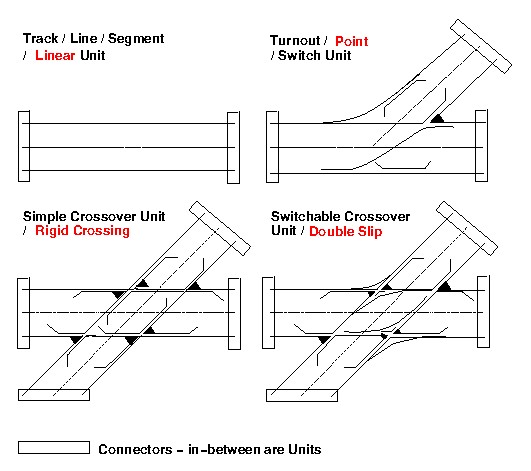
\epsfig{file=rail1.eps,height=\pos{5.4}{11}cm} \ \ 
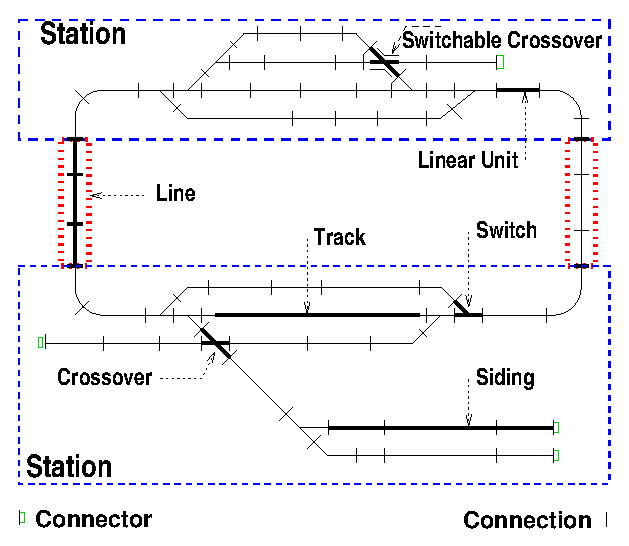
\epsfig{file=rail2.eps,height=\pos{5.4}{9}cm} {[\sort{R}]} 
\caption{{L}eft: Four net units (\textsf{LU, PU, SU, DU}); {R}ight: A railway
  net}\label{fig.railway-net} 
\end{center}
\end{figure}

\mnewfoil

\treprikker

\prinmeth{Pedantic Steps of Development}{primer:pedantic}{%
\begynd
\pind This section, i.e., Sect.\,\ref{sec:Parts}, has illustrated \nyl a principle
      of ``small, pedantic'' analysis \& description steps.
\begynd
\pind You could also call it a principle of separation of concerns\dbsquare
\afslut
\afslut}

\label{before:Ontology and Taxonomy}

\pos{}{%%

\mnewfoil

\vfill
\label{lect2:synth}
\vfill\vspace*{10mm}
\centerline{\lilacolor{Day \#{3}: External Qualities, Synthesis (II)}}
\vfill

}%%%%%%%%

\nbbb{Ontology and Taxonomy}\label{Ontology and Taxonomy}

\begynd
\pind We can speak of two kinds of ontologies\ysf{\footnote{Ontology:
    a set of concepts and categories in a subject area or domain that
    shows their properties and the relations between them [\texttt{Internet}].}}: 
\begynd
\pind the general ontologies of domain analysis \& description, cf.\,Fig.\,\vref{onto.fig2}, and
\pind a specific domain's possible endurant ontologies.
\pind We shall here focus on a [``restricted''] concept of
taxonomies.\footnote{Taxonomy:  a scheme of classification,
      especially a hierarchical classification, in which things are
      organized into groups \wiki.}
\afslut
\afslut

\noindent
\mnewfoil
\bookdefn{Domain Taxonomy}{ By a domain taxonomy we shall understand
\begynd
\pind a hierarchical structure, \nyl usually depicted as a(n
      ``upside-down'') tree,
\pind whose ``root'' designates a compound part
\pind and whose ``siblings'' (proper sub-trees) \nyl designate parts or fluids \dbsquare
\afslut} %%%***

\noindent
\begynd
\pind The `restriction' amounts to considering only endurants.
\pind That is, not considering perdurants.
\pind \isatech{Taxonomy}
\afslut



\noindent
\mnewfoil
\monoexample{The Road Transport System Taxonomy}{%
\begynd
\pind Figure\,\vref{rts.ontology} shows a schematised, i.e., the
      \ldots, taxonomy \nyl
      for the \sfsl{Road Transport System} domain \nyl of Example\,\vref{eks:SoaRTSUoD}.
\afslut
}

\pos{\DBfigure{rts-ontology}{\pos{50mm}{70mm}}{A Road Transport System Taxonomy\dbsquare}{rts.ontology}}
{
 \begin{figure}[h]
  \begin{center}
    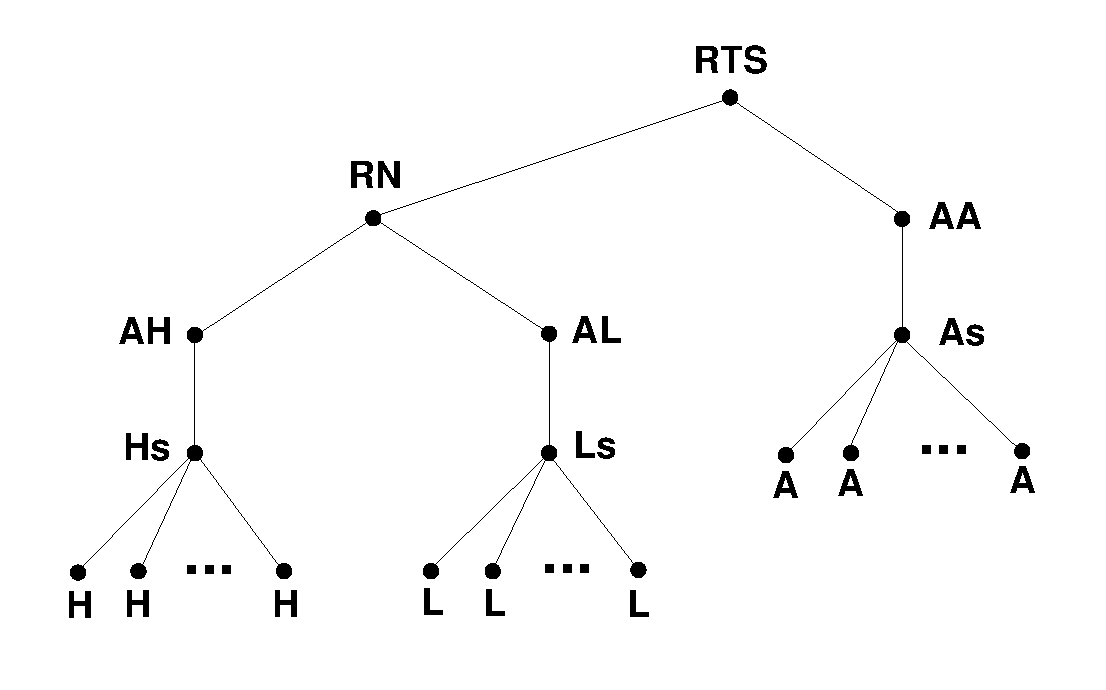
\epsfig{file=rts-ontology.eps,height=\pos{75}{90}mm}
    \caption{A Road Transport System Ontology \dbsquare}\label{rts.ontology}
  \end{center}
\end{figure}
}

\nbbb{``Root'' and ``Sibling'' Parts}\label{Root and Sibling Parts}

\begynd
\pind For compound parts, cf.\,Sect.\,\vref{sec:Compound Parts}, %%%+++
\begynd
\pind we introduce the specific domain taxonomy concepts of ``root'' and ``sibling'' parts.
\pind (We also refer to Fig.\,\vref{rts.ontology}.)
\afslut

\pind When observing, as a human, a compound part\ysf{,} \nyl one may ask the question
\begynd
\pind \sfsl{``a tree \ysf{---} consisting of a specific domain taxonomy node
      labelled, e.g., $X$
\pind and the sub-trees labelled, e.g., $Y_1, Y_2, \ldots, Y_n$ \ysf{---}
\pind does that tree designate one ``indivisible'' part
\pind or does it designate $n+1$ parts\,?''}
\pind We shall, in general, consider the answer to be the latter: $n+1$\,!
\afslut
\afslut

\mnewfoil

\begynd
\pind We shall, in general, consider compound parts to consist of
\begynd
\pind a ``root'' part\ysf{}
\pind and $n$ ``sibling parts and fluids''.
\afslut
\pind What the \ysf{domain modeller} observes
\begynd
\pind appear\ysf{} as one part, ``the whole'',
\pind with $n$ ``embedded'' sub-parts.
\afslut
\pind What the \ysf{domain modeller} is asked to model is
\begynd
\pind $1$, the root part, and
\pind $n$, the sibling\ysf{} parts and fluids.
\afslut
\mnewfoil
\pind The fact that the root part is separately modelled from the sibling parts,
\pind may seem to disappear in this separate modelling ---
\pind but, as You shall see, in the next chapter,
\begynd
\pind their relation: the siblings to ``the whole'', i.e., the root,
\pind will be modelled, specifically through their mereologies,
\pind as will be covered in Sect.\,\ref{chap4.Mereology},
\pind but also through their respective attributes, Sect.\,\ref{chap4.Attributes}.
\afslut
\pind We shall see this non-embbedness of root and sibling parts
\begynd
\pind further accentuated in the modelling of their transcendentally deduced
\pind respective (perdurant) behaviours as distinct concurrent behaviours
\pind in Chapter\,\ref{chap6.tex.1}.
\afslut
\afslut

\label{before:sec:Living Species}

\nbbbb{Living Species}\label{sec:Living Species}

\begynd
\pind \bbcolor{\sfsl{Living Species}} are
\begynd
\pind either \lilacolor{\sfsl{plants}} 
\pind or \lilacolor{\sfsl{animals}}.
\afslut
\pind Among animals we have the \bmcolor{\sfsl{humans}}.
\afslut
\mnewfoil

\nbookdefn{Living Species}{ \label{LivingSpeciesIx}
\begynd
\pind  By a \sfsl{living species} we shall understand \LLLL
\begynd
\pind a solid endurant,
\pind subject to laws of physics, and
\pind additionally subject to \sfsl{causality of
      purpose}. 
\afslut \HHHH
    
\pind Living species
\begynd \LLLL
\pind must have some \sfsl{form they can be developed to reach};
\pind a form they must be \sfsl{causally  determined  to maintain}.
\pind This \sfsl{development and maintenance} must further \nyl engage
      in \sfsl{exchanges of matter with an environment}.
\afslut \HHHH
\pind It must be possible that living species occur in two forms:
\begynd \LLLL
\pind \brcolor{plants}, respectively \brcolor{animals}, 
\pind forms which are characterised by  \nyl \sfsl{development, form and exchange},
\pind which, {additionally}, can be characterised by
\nyl  the \sfsl{ability of purposeful movement}
\ysf{\cite[Kai S{\o}rlander]{kaisorlander1994,kaisorlander1997,kaisorlander2002,kaisorlander2016,kaisorlander2022}}
\dbsquare 
\afslut \HHHH
\afslut
}

\mnewfoil

\newdaprompt{is\_living\_species}{is living species}{$\ell$}{living
  species}{a living species}

\noindent
\isatool{is\_living\_species}

\mnewfoil
\begynd
\pind It is appropriate here to mention \sort{Carl Linnaeus} (1707--1778).
\begynd
\pind He was a Swedish botanist, zoologist, and physician 
\pind who formalised, in the form of a binomial nomenclature, 
\pind the modern system of naming organisms. 
\pind He is known as the ``father of modern taxonomy''.
\pind We refer to his \textsf{`Species Plantarum'} \nyl
      \bbcolor{\texttt{gutenberg.org/files/20771/20771-h/20771-h.htm}}. 
\afslut
\afslut

\nbbb{Plants}\label{sec:Plants}

\monoexample{Plants}{\HHHH%
\begynd
\pind Although we have not yet come across domains for which \nyl the need
      to model the living species of plants were needed, \nyl we give
      some examples anyway:
\begynd
\pind grass,
\pind tulip,
\pind rhododendron,
\pind oak tree.
\afslut
\afslut
}
\mnewfoil

\newdaprompt{is\_plant}{is plant}{$\ell$}{a plant}{a plant}

\noindent
\begynd
\pind \isatool{is\_plant}
\pind The predicate \texttt{is\_living\_species($\ell$)} is a
      prerequisite for \texttt{is\_plant($\ell$)}.
\afslut
      

\nbbb{Animals}\label{sec:Animals}

\nbookdefn{Animal}{ We refer to the initial definition of \sfsl{living
    species} above -- while emphasizing the following traits:
\begynd
\pind (i) a \sfsl{form that animals can be developed to reach} and
\pind (ii)  \sfsl{causally  determined  to  maintain} through
\pind (iii) \sfsl{development and maintenance} \nyl in
      an \sfsl{exchange of matter with an environment}, and
\pind (iv) \sfsl{ability \ysfchgii{of } purposeful movement}
\ysf{\cite[Kai S{\o}rlander]{kaisorlander1994,kaisorlander1997,kaisorlander2002,kaisorlander2016,kaisorlander2022}} \eod
\afslut}

\mnewfoil\pos{\vspace*{-4mm}}{}%t
\newdaprompt{is\_animal}{is animal}{$\ell$}{an animal}{an animal}

\noindent
\begynd
\pind \isatool{is\_animal}
\pind The predicate \texttt{is\_living\_species($\ell$)} is a
      prerequisite for \texttt{is\_animal($\ell$)}.
\pind We distinguish, motivated by \cite[Kai
      S{\o}rlander]{kaisorlander1994,kaisorlander1997,kaisorlander2002,kaisorlander2016,kaisorlander2022},
      between 
\begynd
\pind humans and
\pind other.
\afslut
\afslut

\nbb{Humans}\label{sec:Humans}

\nbookdefn{Human}{
\begynd
\pind A \sfsl{human} (a \sfsl{person}) is an \sfsl{animal}, \nyl
      cf.\,Definition\,\vref{def:Animal},  \nyl with the additional
      properties of having 
\begynd
\pind \sfsl{language},
\pind being \sfsl{conscious} of \sfsl{having knowledge} (of its own
      situation), and
\pind \sfsl{responsibility} \cite[Kai
S{\o}rlander]{kaisorlander1994,kaisorlander1997,kaisorlander2002,kaisorlander2016,kaisorlander2022}
\dbsquare
\afslut
\afslut}

\mnewfoil\pos{\vspace*{-4mm}}{}%t%

\HHHH
\newdaprompt{is\_human}{is human}{$\ell$}{a human}{a human}%
\noindent\HHHH%
\begynd 
\pind \isatool{is\_human}
\pind The predicate \texttt{is\_animal($\ell$)} is a
      prerequisite for \texttt{is\_human($\ell$)}.
\afslut
\mnewfoil\HHHH

\begynd
\pind We have not, \nyl in our many experimental domain modelling efforts
\begynd
\pind had occasion to model humans;
\pind or rather:
\begynd
\pind we have modelled, for example, automobiles
\begynd
\pind as possessing human qualities, 
\pind i.e., ``subsuming humans''.
\afslut
\afslut
\afslut
\mnewfoil
\pind We have found, \nyl  in these experimental domain modelling efforts
\begynd
\pind that we often confer anthropomorphic qualities on artefacts, 
\pind that is, that these artefacts have human characteristics.
\afslut
\pind You, the \pos{readers}{listeners}, are reminded
\begynd
\pind that when some programmers try to explain their programs
\pind they do so using such phrases as
\pind \sfsl{and here the program does ...} so-and-so\,!
\afslut
\afslut

\nbb{Other}\label{sec:Other}

\begynd
\pind We shall skip any treatment of other than human animals\,!
\afslut
\label{chapter1-phy-liv.n}

\treprikker

\noindent
\isaproc{External Quality Analysis \& Description First}

\nbbbbb{Some Observations}\label{Some Observations}

\begynd
\pind Two observations must be made.
 
\begynd
\pind (i) The domain \ysf{modelling} procedures
\begynd
\pind illustrated by
      the analysis functions
\pind  \texttt{de\-term\-ine\_\-Car\-te\-si\-an\_\-parts,
\pind 
      de\-term\-ine\_\-single\_\-sort\_\-part\_set} and
\pind 
      \texttt{de\-term\-ine\_\-al\-tern\-a\-tive\_\-sorts\_\-part\_\-set}
\pind  yield names of
      endurant sorts.
\pind  Some of these names may have already been
      encountered, i.e., discovered.
\pind  That is, the domain \ysf{modeller} must
      carefully consider such possibilities.
\afslut
      
\mnewfoil

\pind (ii) Endurants are \sort{\underline{not}\ recursively definable}\,! 
\begynd
\pind This appears to come as a surprise \nyl to many computer scientists.
\pind Immediately many suggest that ``tree-like'' endurants  \nyl like a river,
\pind or, indeed, a tree, 
\pind should be defined recursively.
\pind But we posit that that is not the case.
\pind A river, for example, has a delta, its ``root'' so-to-speak,
\pind but the sub-trees of a recursively defined river endurant
\pind ha\ysfchg{ve } no such ``deltas''\,! 
\pind Instead we define such
      ``tree-like'' endurants \nyl  as graphs with appropriate
      mereologies \ysf{-- as introduced in the next chapter}.
\afslut
\afslut
\afslut

\label{lect2.label.analysis}


\nbbbbb{States}\label{A Part State}\label{kap3.States.general}\label{lect2.label.synthesis} 

\begynd
\pind In our continued modelling
\begynd
\pind we shall make good use of a concept of states.
\afslut
\afslut

\pos{\vspace*{2mm}}{\vspace*{2cm}}

\bookdefn{State, II}{By a \sfsl{state} we shall understand
\begynd
\pind any collection of one or more parts \dbsquare\
\afslut}
\noindent%
\pos{\psno}{\mnewfoil}%
\begynd%
\pind In Chapter\,\ref{chap4.tex.1} Sect.\,\ref{chap4.Attributes} \nyl
we introduce the notion of \sfsl{attributes.} 
\begynd
\pind Among attributes there are the \sfsl{dynamic attributes}.
\pind They model that internal \ysf{} quality values \nyl  may change dynamically.
\pind So we may wish, on occasion, to `refine' our notion of state
      \nyl to be just those parts which have dynamic attributes.
\afslut
\afslut

\nbbbb{State Calculation}\label{kap3.State Calculation}\label{kap3-gen-state}
\begynd
\pind Given any universe of discourse, \textsf{uod:UoD}, we can
      recursively calculate its ``full'' state, \textsf{calc\_parts({\LBRACE}uod{\RBRACE})}.
\afslut\LLll
\begin{enumerate}\setei
\item \label{uod:state:000} Let \textsf{e} be any endurant. \dbeat{\\}
      Let \textsf{arg\_parts} be the parts to be calculated. \dbeat{\\}
      Let \textsf{res\_parts} be the parts calculated. \dbeat{\\}
      Initialise the \textsf{calc}ulator with
      \textsf{arg\_parts=$\{$uod$\}$} and \textsf{res\_parts=$\{\}$}. \dbeat{\\}
      Calculation stops with \textsf{arg\_parts} empty and
      \textsf{res\_parts} the result.
\item \label{uod:state:010} If  \texttt{is\_Cartesian}(\textsf{e})  
\item \label{uod:state:010a}  then we obtain its
      immediate parts, \textsf{determine\_com\-po\-site\_\-part(e)}
\item \label{uod:state:010b} add them, as a set, to \textsf{arg\_parts}, \textsf{e}
      removed from  \textsf{arg\_parts} and added to
      \textsf{res\_parts} calculating the parts from that.
\item \label{uod:state:012} If 
      \texttt{is\_single\_sort\_part\_set}(\textsf{e}) 
\item \label{uod:state:013} then the parts,
      \textsf{ps}, of the single sort set are determined, 
\item \label{uod:state:014} added to \textsf{arg\_parts} and \textsf{e}
      removed from  \textsf{arg\_parts} and added to
      \textsf{res\_parts} calculating the parts from that.
\item \label{uod:state:016} If
      \texttt{is\_alternative\_sorts\_part\_set}(\textsf{e}) then the
      parts, \textsf{((p1,\_),(p2,\_),...,(pn,\_))}, of 
      the alternative sorts set are determined, added to \textsf{arg\_parts} and \textsf{e}
      removed from  \textsf{arg\_parts} and added to  \textsf{res\_parts} calculating the parts from that.
\savei\end{enumerate}
\pos{\psno}{\mnewfoil}
\noindent
\pos{\doafpr\afindex{calc\_parts}\psno}{\mnewfoil}\pos{}{\normalsize\HHHH\sf}
%\RSLatex
%value
%&\ref{uod:state:000}.&   calc_parts: E-set -> E-set -> E-set
%&\ref{uod:state:000}.&   calc_parts(arg_parts)(res_parts) is
%&\ref{uod:state:000}.&      if arg_parts = {} then res_parts else
%&\ref{uod:state:000}.&      let e :- e isin arg_parts in
%&\ref{uod:state:010}.&      is_Cartesian(e) -> 
%&\ref{uod:state:010a}.&          let ((e1,e2,...,en),_) = observe_Cartesian_part(e) in 
%&\ref{uod:state:010b}.&          calc_parts(arg_parts\{e} union {e1,e2,...,en})(res_parts union {e}) end
%&\ref{uod:state:012}.&      is_single_sort_part_set(e) ->   
%&\ref{uod:state:013}.&          let ps = observe_single_sort_part_set(e) in 
%&\ref{uod:state:014}.&          calc_parts(arg_parts\{e}union ps)(res_parts union {e}) end
%&\ref{uod:state:016}.&      is_alternative_sort_part_set(e) ->    
%&\ref{uod:state:016}.&          let ((p1,_),(p2,_),...,(pn,_)) = observe_alternative_sorts_part_set(e) in 
%&\ref{uod:state:016}.&          calc_parts(arg_parts\{e}union{p1,p2,...,pn})(res_parts union {e}) end
%&\ref{uod:state:000}.&      end end
%\endRSLatex 
\bp
\kw{value}\\
\ref{uod:state:000}.\ \ \ calc\_parts: E\kw{-set} {\RIGHTARROW} E\kw{-set} {\RIGHTARROW} E\kw{-set}\\
\ref{uod:state:000}.\ \ \ calc\_parts(arg\_parts)(res\_parts) {\IS}\\
\ref{uod:state:000}.\ \ \ \ \ \ \kw{if} arg\_parts {\EQ} {\LBRACE}{\RBRACE} \kw{then} res\_parts \kw{else}\\
\ref{uod:state:000}.\ \ \ \ \ \ \kw{let} e {\RDOT} e {\ISIN} arg\_parts \kw{in}\\
\ref{uod:state:010}.\ \ \ \ \ \ is\_Cartesian(e) {\RIGHTARROW} \\
\ref{uod:state:010a}.\ \ \ \ \ \ \ \ \ \ \kw{let} ((e1,e2,{\DOTDOTDOT},en),{\UNDERLINE}) {\EQ} observe\_Cartesian\_part(e) \kw{in} \\
\ref{uod:state:010b}.\ \ \ \ \ \ \ \ \ \ calc\_parts(arg\_parts{\SETMINUS}{\LBRACE}e{\RBRACE} {\UNION} {\LBRACE}e1,e2,{\DOTDOTDOT},en{\RBRACE})(res\_parts {\UNION} {\LBRACE}e{\RBRACE}) \kw{end}\\
\ref{uod:state:012}.\ \ \ \ \ \ is\_single\_sort\_part\_set(e) {\RIGHTARROW}\ \ \ \\
\ref{uod:state:013}.\ \ \ \ \ \ \ \ \ \ \kw{let} ps {\EQ} observe\_single\_sort\_part\_set(e) \kw{in} \\
\ref{uod:state:014}.\ \ \ \ \ \ \ \ \ \ calc\_parts(arg\_parts{\SETMINUS}{\LBRACE}e{\RBRACE}{\UNION} ps)(res\_parts {\UNION} {\LBRACE}e{\RBRACE}) \kw{end}\\
\ref{uod:state:016}.\ \ \ \ \ \ is\_alternative\_sort\_part\_set(e) {\RIGHTARROW}\ \ \ \ \\
\ref{uod:state:016}.\ \ \ \ \ \ \ \ \ \ \kw{let} ((p1,{\UNDERLINE}),(p2,{\UNDERLINE}),{\DOTDOTDOT},(pn,{\UNDERLINE})) {\EQ} observe\_alternative\_sorts\_part\_set(e) \kw{in} \\
\ref{uod:state:016}.\ \ \ \ \ \ \ \ \ \ calc\_parts(arg\_parts{\SETMINUS}{\LBRACE}e{\RBRACE}{\UNION}{\LBRACE}p1,p2,{\DOTDOTDOT},pn{\RBRACE})(res\_parts {\UNION} {\LBRACE}e{\RBRACE}) \kw{end}\\
\ref{uod:state:000}.\ \ \ \ \ \ \kw{end} \kw{end}
\ep
\pos{\rm}{}

\noindent
\isatool{calc\_parts}

\pos{\psno}{\mnewfoil}

\prinmeth{Domain State}{meth:domain-state}{%
\begynd
\pind We have found, once all the state components, \nyl i.e.,
      the endurant parts, \nyl have had their external qualities
      analysed, that
\begynd
\pind it is then expedient to define the domain state.
\pind It can then be the basis for several concepts 
\pind of internal qualities.
\afslut
\afslut}

\pos{\psno}{\mnewfoil}
\monoexample{Constants and States}{
\begin{enumerate}\setei
\item \label{srares-000} Let there be given a universe of discourse,
                         $rts$ (\ysfchg{Road Transport System}). \nyl The set $\{rts\}$ is an example of a state.
\savei\end{enumerate}
\noindent From that state we can calculate other states.

\begin{enumerate}\setei
\item \label{srares-020} The set of all hubs, $hs$. \vidxi{$hs$}{srares-020} 
\item \label{srares-030} The set of all links, $ls$. \vidxi{$ls$}{srares-030} 
\item \label{srares-040} The set of all hubs and links, $hls$. \vidxi{$hls$}{srares-040} 
\item \label{srares-080} The set of all automobiles, $as$. \vidxi{$as$}{srares-080} 
\item \label{srares-090} The set of all parts, $ps$.\vidxi{$ps$}{srares-090} 
\savei\end{enumerate}
\pos{\psno}{\mnewfoil}\ysfchgii{
%\RSLatex
%value
%&\ref{srares-000}&   &$rts$&:UoD
%&\ref{srares-020}&   &$hs$&:H-set  is obs_sH(obs_SH(obs_RN(&$rts$&)))
%&\ref{srares-030}&   &$ls$&:L-set is obs_sL(obs_SL(obs_RN(&$rts$&)))
%&\ref{srares-040}&   &$hls$&:(H|L)-set is &$hs$& union &$ls$&  
%&\ref{srares-080}&   &$as$&:A-set is obs_As(obs_AA(obs_RN(&$rts$&)))
%&\ref{srares-090}&   &$ps$&:(&\ysfchgii{UoD}&|H|L|A)-set is &$rts$& union &$hls$& union &$as$  \eod&
%\endRSLatex    
\bp
\kw{value}\\
\ref{srares-000}\ \ \ $rts$:UoD\\
\ref{srares-020}\ \ \ $hs$:H\kw{-set}\ \ {\IS} obs\_sH(obs\_SH(obs\_RN($rts$)))\\
\ref{srares-030}\ \ \ $ls$:L\kw{-set} {\IS} obs\_sL(obs\_SL(obs\_RN($rts$)))\\
\ref{srares-040}\ \ \ $hls$:(H{\BAR}L)\kw{-set} {\IS} $hs$ {\UNION} $ls$\ \ \\
\ref{srares-080}\ \ \ $as$:A\kw{-set} {\IS} obs\_As(obs\_AA(obs\_RN($rts$)))\\
\ref{srares-090}\ \ \ $ps$:({UoD}{\BAR}H{\BAR}L{\BAR}A)\kw{-set} {\IS} $rts$ {\UNION} $hls$ {\UNION} $as$  \eod
\ep
}}\eysf

\nbbbb{Updateable States}\label{kap3.States.specific}

\begynd
\pind We shall, in Sect.\,\ref{chap4.Attributes}, introduce the notion of parts,
\begynd
\pind having dynamic attributes,
\pind that is, having internal qualities that may change.
\afslut
\pind To cope with the modelling, 
\pind in particular of so-called \sfsl{monitor-able} attributes,
\pind we present the \sfsl{state} as a global variable:
\afslut


%\RSLatex
%variable `sigma := calc_parts({uod})
%\endRSLatex 
\bp
\kw{variable} $\sigma$ :{\EQ} calc\_parts({\LBRACE}uod{\RBRACE})
\ep


\nbbbbb{An External Analysis and Description Procedure}\label{External Analysis and Description Procedure}

\begynd
\pind We have covered 
\begynd
\pind the individual analysis and description steps
\pind of our approach to the external qualities modelling 
\pind of domain endurants. 
\afslut
\pind We now suggest
\begynd 
\pind a `formal' description of the process
\pind of linking all these analysis and description steps.
\afslut
\afslut

\nbbbb{An Analysis \& Description State}\label{A Description State}\label{ADomainDiscoveryNoticeBoard}

\begynd
\pind Common to all the discovery processes is an idea of a
      \sfsl{notice board}. 
\pind A notice board, at any time in the development of a domain
      description,  is a repository of the analysis and description process. 
\pind We suggest to model the notice board in terms of \ysf{four} global
      variables.
\begynd
\pind The \bbcolor{\textsf{new}} variable holds the \bmcolor{parts} yet to be described;
\pind the \bbcolor{\textsf{ans}} variable holds the \bmcolor{sort
      name\ysfchg{s } of parts} that have so far been
      described;
\pind the \bbcolor{\textsf{gen}} variable holds the \bmcolor{parts} that have so far been
      described; and
\pind the \bbcolor{\textsf{txt}} variable holds the \bmcolor{\rsltxt} so far generated.
\begynd
\pind We model  the \bbcolor{\textsf{txt}} variable as a  map 
\pind from endurant identifier names to \bmcolor{\rsltxt}.
\afslut
\afslut
\afslut\HHHH
\pos{\psno}{\mnewfoil}

\vspace*{2mm}

\boiteepaisseavecuntitre{Discovery Schema 0: The Notice Board}
\label{DiscoverySchema0}\label{A Domain Discovery Notice Board}
%\RSLatex
%variable
%   new := {uod} ,
%   asn := { &\bq& UoD &\eq& }
%   gen := {} ,
%   txt:&\rsltxt&  := [ uid_UoD(uod) +> <.&\bq&type UoD&\eq&.> ]
%\endRSLatex
\bp
\kw{variable}\\
\>\ new :{\EQ} {\LBRACE}uod{\RBRACE} ,\\
\>\ asn :{\EQ} {\LBRACE} \bq UoD \eq {\RBRACE}\\
\>\ gen :{\EQ} {\LBRACE}{\RBRACE} ,\\
\>\ txt:\rsltxt\ \ :{\EQ} {\LBRACKET} uid\_UoD(uod) {\MAPSTO} {\LANGLE}\bq\kw{type} UoD\eq{\RANGLE} {\RBRACKET}
\ep
\endboiteepaisseavecuntitre\pos{\normalsize}{\HHHH}\rm


\nbbbb{A Domain Discovery Procedure, I}\label{The Procedure}\label{A Domain Discovery Process, I}
 
\begynd
\pind The \textsf{discover\_sorts} pseudo program
\begynd
\pind suggests a systematic way of proceeding
\pind through analysis, manifested by the \textsf{is\_$\cdots$} predicates,
\pind to ({\RIGHTARROW}) description.
\afslut
\afslut

\begynd
\pind Some comments are in order.
\begynd
\pind The \textsf{e-set$_a$}$\sqcupplus$\textsf{e-set$_b$} expression
\pind yields a set of endurants that are either in \textsf{e-set$_a$},
      or in \textsf{e-set$_a$}, or in both,
\pind but such that two endurants, \textsf{e$_x$} and \textsf{e$_y$}
\pind which are of the same endurant\ysfchg{ } type, say \textsf{E}, 
\pind and are in respective sets is only represented once in the
      result\ysfchg{. }\dbeat{ 
\pind that is, if they are type-wise the same, but value-wise different
\pind they will only be included once in the result.}
\afslut
                                \pos{\psno}{\mnewfoil}\HHHH

\pind As this is the first time \rsltxt\ is put on the notice board \nyl we express this as:
\begin{itemize}
\item \textsf{txt :{\EQ} txt {\UNION} {\LBRACKET}type\_name(v) {\MAPSTO} {\LANGLE}\rsltxt{\RANGLE}{\RBRACKET}}
\end{itemize}
\pind Subsequent insertion of \rsltxt\ \nyl for internal quality
descriptions and perdurants  \nyl is then concatenated to the end of
previously uploaded \rsltxt.
\afslut

\pos{\psno\vspace*{4mm}}{\mnewfoil \vspace*{-4mm}}

\boiteepaisseavecuntitre{\LLll \ysf{Discovery Schema 1: An
    External Qualities Domain Modelling} Process} \label{DiscoverySchema1}
\LLll
  
\pos{\footnotesize\small\normalsize}{\Large}\label{discover-sorts}
%\RSLatex
%value
% discover_sorts: Unit -> Unit
% discover_sorts() is while new ~= {} do 
%   let v :- v isin new in (new := new \ {v} || gen := gen union {v} || ans := ans \ {type_of(v)}) ;
%   is_atomic(v) -> skip ,
%   is_compound(v) ->
%    is_Cartesian(v) ->
%     let ((e1,...,en),(&$\eta$E1,...,$\eta$En&))=determine_Cartesian_part_sorts(v) in&\afindex{determine\_Cartesian\_part\_sorts}&
%     (ans := ans union {&$\eta$E1,...,$\eta$En&} || new := new &$\sqcupplus$& {e1,...,en}  
%      || txt := txt union [type_name(v) +> <.describe_Cartesian_part_sorts(v).>]) end,&\dpindex{describe\_Cartesian\_part\_sorts}& 
%    is_part_set(v) ->
%     let ({p1,...,pn},&$\eta$P&)=determine_part_set_sort(v) in&\afindex{determine\_part\_set\_sort}&
%     (ans := ans union {&$\eta$P&} || new := new &$\sqcupplus$& {p1,...,pn} ||
%      txt := txt union [type_name(v) +> describe_part_set_sort(v)]) end,&\dpindex{describe\_part\_set\_sort}& 
%  end end
%\endRSLatex
\bp
\kw{value}\\
 discover\_sorts: \kw{Unit} {\RIGHTARROW} \kw{Unit}\\
 discover\_sorts() {\IS} \kw{while} new {\NOTEQ} {\LBRACE}{\RBRACE} \kw{do} \\
\>\ \kw{let} v {\RDOT} v {\ISIN} new \kw{in} (new :{\EQ} new {\SETMINUS} {\LBRACE}v{\RBRACE} {\PARL} gen :{\EQ} gen {\UNION} {\LBRACE}v{\RBRACE} {\PARL} ans :{\EQ} ans {\SETMINUS} {\LBRACE}type\_of(v){\RBRACE}) ;\\
\>\ is\_atomic(v) {\RIGHTARROW} \kw{skip} ,\\
\>\ is\_compound(v) {\RIGHTARROW}\\
\>\>is\_Cartesian(v) {\RIGHTARROW}\\
\>\>\ \kw{let} ((e1,{\DOTDOTDOT},en),($\eta$E1,...,$\eta$En)){\EQ}determine\_Cartesian\_part\_sorts(v) \kw{in}\afindex{determine\_Cartesian\_part\_sorts}\\
\>\>\ (ans :{\EQ} ans {\UNION} {\LBRACE}$\eta$E1,...,$\eta$En{\RBRACE} {\PARL} new :{\EQ} new $\sqcupplus$ {\LBRACE}e1,{\DOTDOTDOT},en{\RBRACE}\ \ \\
\>\>\>{\PARL} txt :{\EQ} txt {\UNION} {\LBRACKET}type\_name(v) {\MAPSTO} {\LANGLE}describe\_Cartesian\_part\_sorts(v){\RANGLE}{\RBRACKET}) \kw{end},\dpindex{describe\_Cartesian\_part\_sorts} \\
\>\>is\_part\_set(v) {\RIGHTARROW}\\
\>\>\ \kw{let} ({\LBRACE}p1,{\DOTDOTDOT},pn{\RBRACE},$\eta$P){\EQ}determine\_part\_set\_sort(v) \kw{in}\afindex{determine\_part\_set\_sort}\\
\>\>\ (ans :{\EQ} ans {\UNION} {\LBRACE}$\eta$P{\RBRACE} {\PARL} new :{\EQ} new $\sqcupplus$ {\LBRACE}p1,{\DOTDOTDOT},pn{\RBRACE} {\PARL}\\
\>\>\>txt :{\EQ} txt {\UNION} {\LBRACKET}type\_name(v) {\MAPSTO} describe\_part\_set\_sort(v){\RBRACKET}) \kw{end},\dpindex{describe\_part\_set\_sort} \\
\>\kw{end} \kw{end}
\ep
\endboiteepaisseavecuntitre\pos{\normalsize}{\HHHH}\rm
\noindent
\pos{\psno}{\mnewfoil}%%%

\pos{\noindent
\isaproc{discover\_sorts}}{}
  
\nbbbbb{Summary}\label{sec:extq.Summary}\label{X:Summary}

\begynd
\pind We briefly summarise the main findings of this \pos{chapter}{lecture}.
\pind These are the main 
\begynd
\pind analysis predicates and functions\ysfchg{, }
      and
\pind  the main description functions.
\afslut
\pind These, to remind the \pos{reader}{student}, are
\begynd
\pind \ysfchg{(i) } the \sfsl{analysis}, the \texttt{is\_$\cdots$}, \sfsl{predicates},
\pind \ysfchg{(ii) }  the \sfsl{analysis}, the \texttt{determine\_$\cdots$},
      \sfsl{functions}, 
\pind \ysfchg{(iii) }  the \sfsl{state calculation} function, 
\pind \ysfchg{(iv) }  the \sfsl{description} functions, and
\pind \ysfchg{(v) }  the \sfsl{domain discovery} procedure.
\afslut
\afslut
\mnewfoil

\pos{
\begynd
\pind They are summarised in this table:
\afslut

\pos{\boiteepaisseavecuntitre{\brcolor{External Qualities Predicates and
Functions: Method Tools}}
\label{functions-table-1}
\begin{minipage}[h]{5.5cm}\sf\small\sf
\begin{quote}
\begin{itemize}
\item \sort{Analysis Predicates:} These are the \texttt{is\_$\cdots$}
  functions. The domain scientist cum engineer, i.e., the domain
  analyser cum describer, applies this to entities being observed in
  the domain. The answer is a truth value. Dependent on the truth value
  that person then goes on to apply, again informally, either a
  subsequent predicate, or some function.
\item \sort{Analysis Functions:} These are the
  \texttt{determine\_$\cdots$} functions. They apply, respectively, to
  parts satisfying respective predicates.
\item \sort{State Calculation:} The state calculation function is
  given generally. The domain analyser cum describer must define this
  function for each domain studied.
\item \sort{Description Functions:} These calculation functions, in a
  sense, are the main ``results'' of this chapter.
\item \sort{Domain Discovery:} The procedure here being described,
  informally, guides the domain analyser cum describer to do the job\,!
\end{itemize}\normalsize
\end{quote}
\end{minipage}
\begin{minipage}[h]{5mm} \ \
\end{minipage}
\begin{minipage}[h]{7cm}\small\sf
\qbtabular\\
%                     
%%%%%%%%%%%%%%%%%%%%%%%%%%%%%%%%%%%%%%%%%%%%%%%%%%%%%%%%%%%%%%%%%%%%%%%
%%%% Released for translation 22 April 2023  %%%%%%%%%%%%%%%%%%%%%%%%%%
%%%%%%%%%%%%%%%%%%%%%%%%%%%%%%%%%%%%%%%%%%%%%%%%%%%%%%%%%%%%%%%%%%%%%%%         %
& \ \ \ \brcolor{Analysis Predicates} & \\
\plineo{dap:is-entity}{is\_entity}{isentity}\\
\plineo{dap:is-endurant}{is\_endurant}{isendurant}\\
\plineo{dap:is-perdurant}{is\_perdurant}{isperdurant}\\
\plineo{dap:is solid}{is\_solid}{issolid}\\
\plineo{dap:is fluid}{is\_fluid}{isfluid}\\
\plineo{dap:is physical part}{is\_part}{isphysicalpart}\\
\plineo{dap:is atomic part}{is\_atomic}{isatomicpart}\\
\plineo{dap:is compound part}{is\_compound}{iscompoundpart}\\
\plineo{dap:is-cartesian}{is\_Cartesian}{iscartesian}\\
\plineo{dap:is-single-sort-set}{is\_part\_set\ysfchg{\_sort}}{issinglesortset}\\
\plineo{dap:is living species}{is\_living\_species}{a living species}\\
\plineo{dap:is plant}{is\_plant}{a plant}\\
\plineo{dap:is animal}{is\_animal}{an animal}\\
\plineo{dap:is human}{is\_human}{a human}\\
& \ \ \ \brcolor{Analysis Functions} & \\
\plineo{dap:analyse-cp}{determine\_Cartesian\_part\_sorts}{determineCartesian}\\
\plineo{dap:determine-single-sort-part-set}{determine\_part\_set\_sort}{DsSpS}\\
& \ \ \ \brcolor{State Calculation} & \\
\pline{calc\_parts}{uod:state:000}\\
& \ \ \ \brcolor{Description Functions} & \\
\plineo{ddp:UoD}{describe\_Universe\_of\_Discourse}{DS1}\\
\plineo{ddp:calc-Cartesian-parts}{describe\_Cartesian\_part\_sorts}{DS2}\\
\plineo{ddp:calc-single-sort-part-set-sorts}{describe\_part\_set\_sort}{DS3}\\
& \ \ \ \brcolor{Domain Discovery} & \\
\pline{discover\_sorts}{discover-sorts}\\

\qetabular\normalsize
\end{minipage}
\endboiteepaisseavecuntitre
%%  LocalWords:  analyser
}{\normalsize\large\large%\vspace*{-15mm}
\qbtabular\\
\pos{}{\large}%                     
%%%%%%%%%%%%%%%%%%%%%%%%%%%%%%%%%%%%%%%%%%%%%%%%%%%%%%%%%%%%%%%%%%%%%%%
%%%% Released for translation 22 April 2023  %%%%%%%%%%%%%%%%%%%%%%%%%%
%%%%%%%%%%%%%%%%%%%%%%%%%%%%%%%%%%%%%%%%%%%%%%%%%%%%%%%%%%%%%%%%%%%%%%%         %
& \ \ \ \brcolor{Analysis Predicates} & \\
\plineo{dap:is-entity}{is\_entity}{isentity}\\
\plineo{dap:is-endurant}{is\_endurant}{isendurant}\\
\plineo{dap:is-perdurant}{is\_perdurant}{isperdurant}\\
\plineo{dap:is solid}{is\_solid}{issolid}\\
\plineo{dap:is fluid}{is\_fluid}{isfluid}\\
\plineo{dap:is physical part}{is\_part}{isphysicalpart}\\
\plineo{dap:is atomic part}{is\_atomic}{isatomicpart}\\
\plineo{dap:is compound part}{is\_compound}{iscompoundpart}\\
\plineo{dap:is-cartesian}{is\_Cartesian}{iscartesian}\\
\plineo{dap:is-single-sort-set}{is\_part\_set\ysfchg{\_sort}}{issinglesortset}\\
\plineo{dap:is living species}{is\_living\_species}{a living species}\\
\plineo{dap:is plant}{is\_plant}{a plant}\\
\plineo{dap:is animal}{is\_animal}{an animal}\\
\plineo{dap:is human}{is\_human}{a human}\\
& \ \ \ \brcolor{Analysis Functions} & \\
\plineo{dap:analyse-cp}{determine\_Cartesian\_part\_sorts}{determineCartesian}\\
\plineo{dap:determine-single-sort-part-set}{determine\_part\_set\_sort}{DsSpS}\\
& \ \ \ \brcolor{State Calculation} & \\
\pline{calc\_parts}{uod:state:000}\\
& \ \ \ \brcolor{Description Functions} & \\
\plineo{ddp:UoD}{describe\_Universe\_of\_Discourse}{DS1}\\
\plineo{ddp:calc-Cartesian-parts}{describe\_Cartesian\_part\_sorts}{DS2}\\
\plineo{ddp:calc-single-sort-part-set-sorts}{describe\_part\_set\_sort}{DS3}\\
& \ \ \ \brcolor{Domain Discovery} & \\
\pline{discover\_sorts}{discover-sorts}\\

\qetabular\HHHH}
}{}

\mnewfoil

\treprikker

\noindent
\begynd
\pind Please consider Fig.\,\ref{onto.fig2} [\pos{Page}{Slide}\,\pageref{onto.fig2}].
\begynd
\pind This \pos{chapter}{lecture} has covered the tree-like structure
      \nyl to the left in  Fig.\,\ref{onto.fig2}.
\pind The next \pos{chapter covers}{lectures cover} the horisontal and
      vertical lines, 
      \nyl also to the left in Fig.\,\ref{onto.fig2}.
\afslut
\afslut
\label{primer-extq.n}

%%  LocalWords:  Endurants analysed analyser endurant RTS priori et
%%  LocalWords:  formalise endurants perdurants perdurant verbed eks
%%  LocalWords:  cetera geo plasmatic compartmentalise fn analyse RSL
%%  LocalWords:  characterisation artefactual atomism analysing wrt
%%  LocalWords:  modelling cartesian po cp Ei Cartesians calc eind SL
%%  LocalWords:  Formalisation Disjointness typenames UoD pts ved un
%%  LocalWords:  cluding ps Pn pn le Hs al tive disjointness NUs SU
%%  LocalWords:  LinU PntU SwiU DblU TerU eft ight characterised www
%%  LocalWords:  formalised gu modelled artefacts txt uod asn uid rts
%%  LocalWords:  ontologies taxonomical schematised labelled arg hs
%%  LocalWords:  Initialise ulator srares hls bcs bs sH sL BCs SBC FV
%%  LocalWords:  bc UoB ddp isphysicalpart isatomicpart iscartesian
%%  LocalWords:  iscompoundpart doaf Defn mereologies embbedness UoDs
%%  LocalWords:  behaviours Plantarum summarise indsnaevring filosofi
%%  LocalWords:  Kai rlander sep Artifactual de ine te si summarised
%%  LocalWords:  horisontal sortness modeller SoaRTSUoD VDM pdefind
%%  LocalWords:  characterises Updateable pconind omments ve
